\begin{figure}[htbp]
\centering

\tikzset{every picture/.style={line width=0.75pt}} %set default line width to 0.75pt        

\begin{tikzpicture}[x=0.75pt,y=0.75pt,yscale=-1,xscale=1]
%uncomment if require: \path (0,688.6666717529297); %set diagram left start at 0, and has height of 688.6666717529297

%Rounded Rect [id:dp5821291554412268] 
\draw  [fill={rgb, 255:red, 242; green, 175; blue, 175 }  ,fill opacity=1 ] (262,215.23) .. controls (262,204.98) and (270.31,196.67) .. (280.57,196.67) -- (494.43,196.67) .. controls (504.69,196.67) and (513,204.98) .. (513,215.23) -- (513,270.93) .. controls (513,281.19) and (504.69,289.5) .. (494.43,289.5) -- (280.57,289.5) .. controls (270.31,289.5) and (262,281.19) .. (262,270.93) -- cycle ;
%Straight Lines [id:da529959831445817] 
\draw    (306,258.5) -- (467,253.67) ;


%Image [id:dp6543088529680775] 
\draw (297,257.5) node  {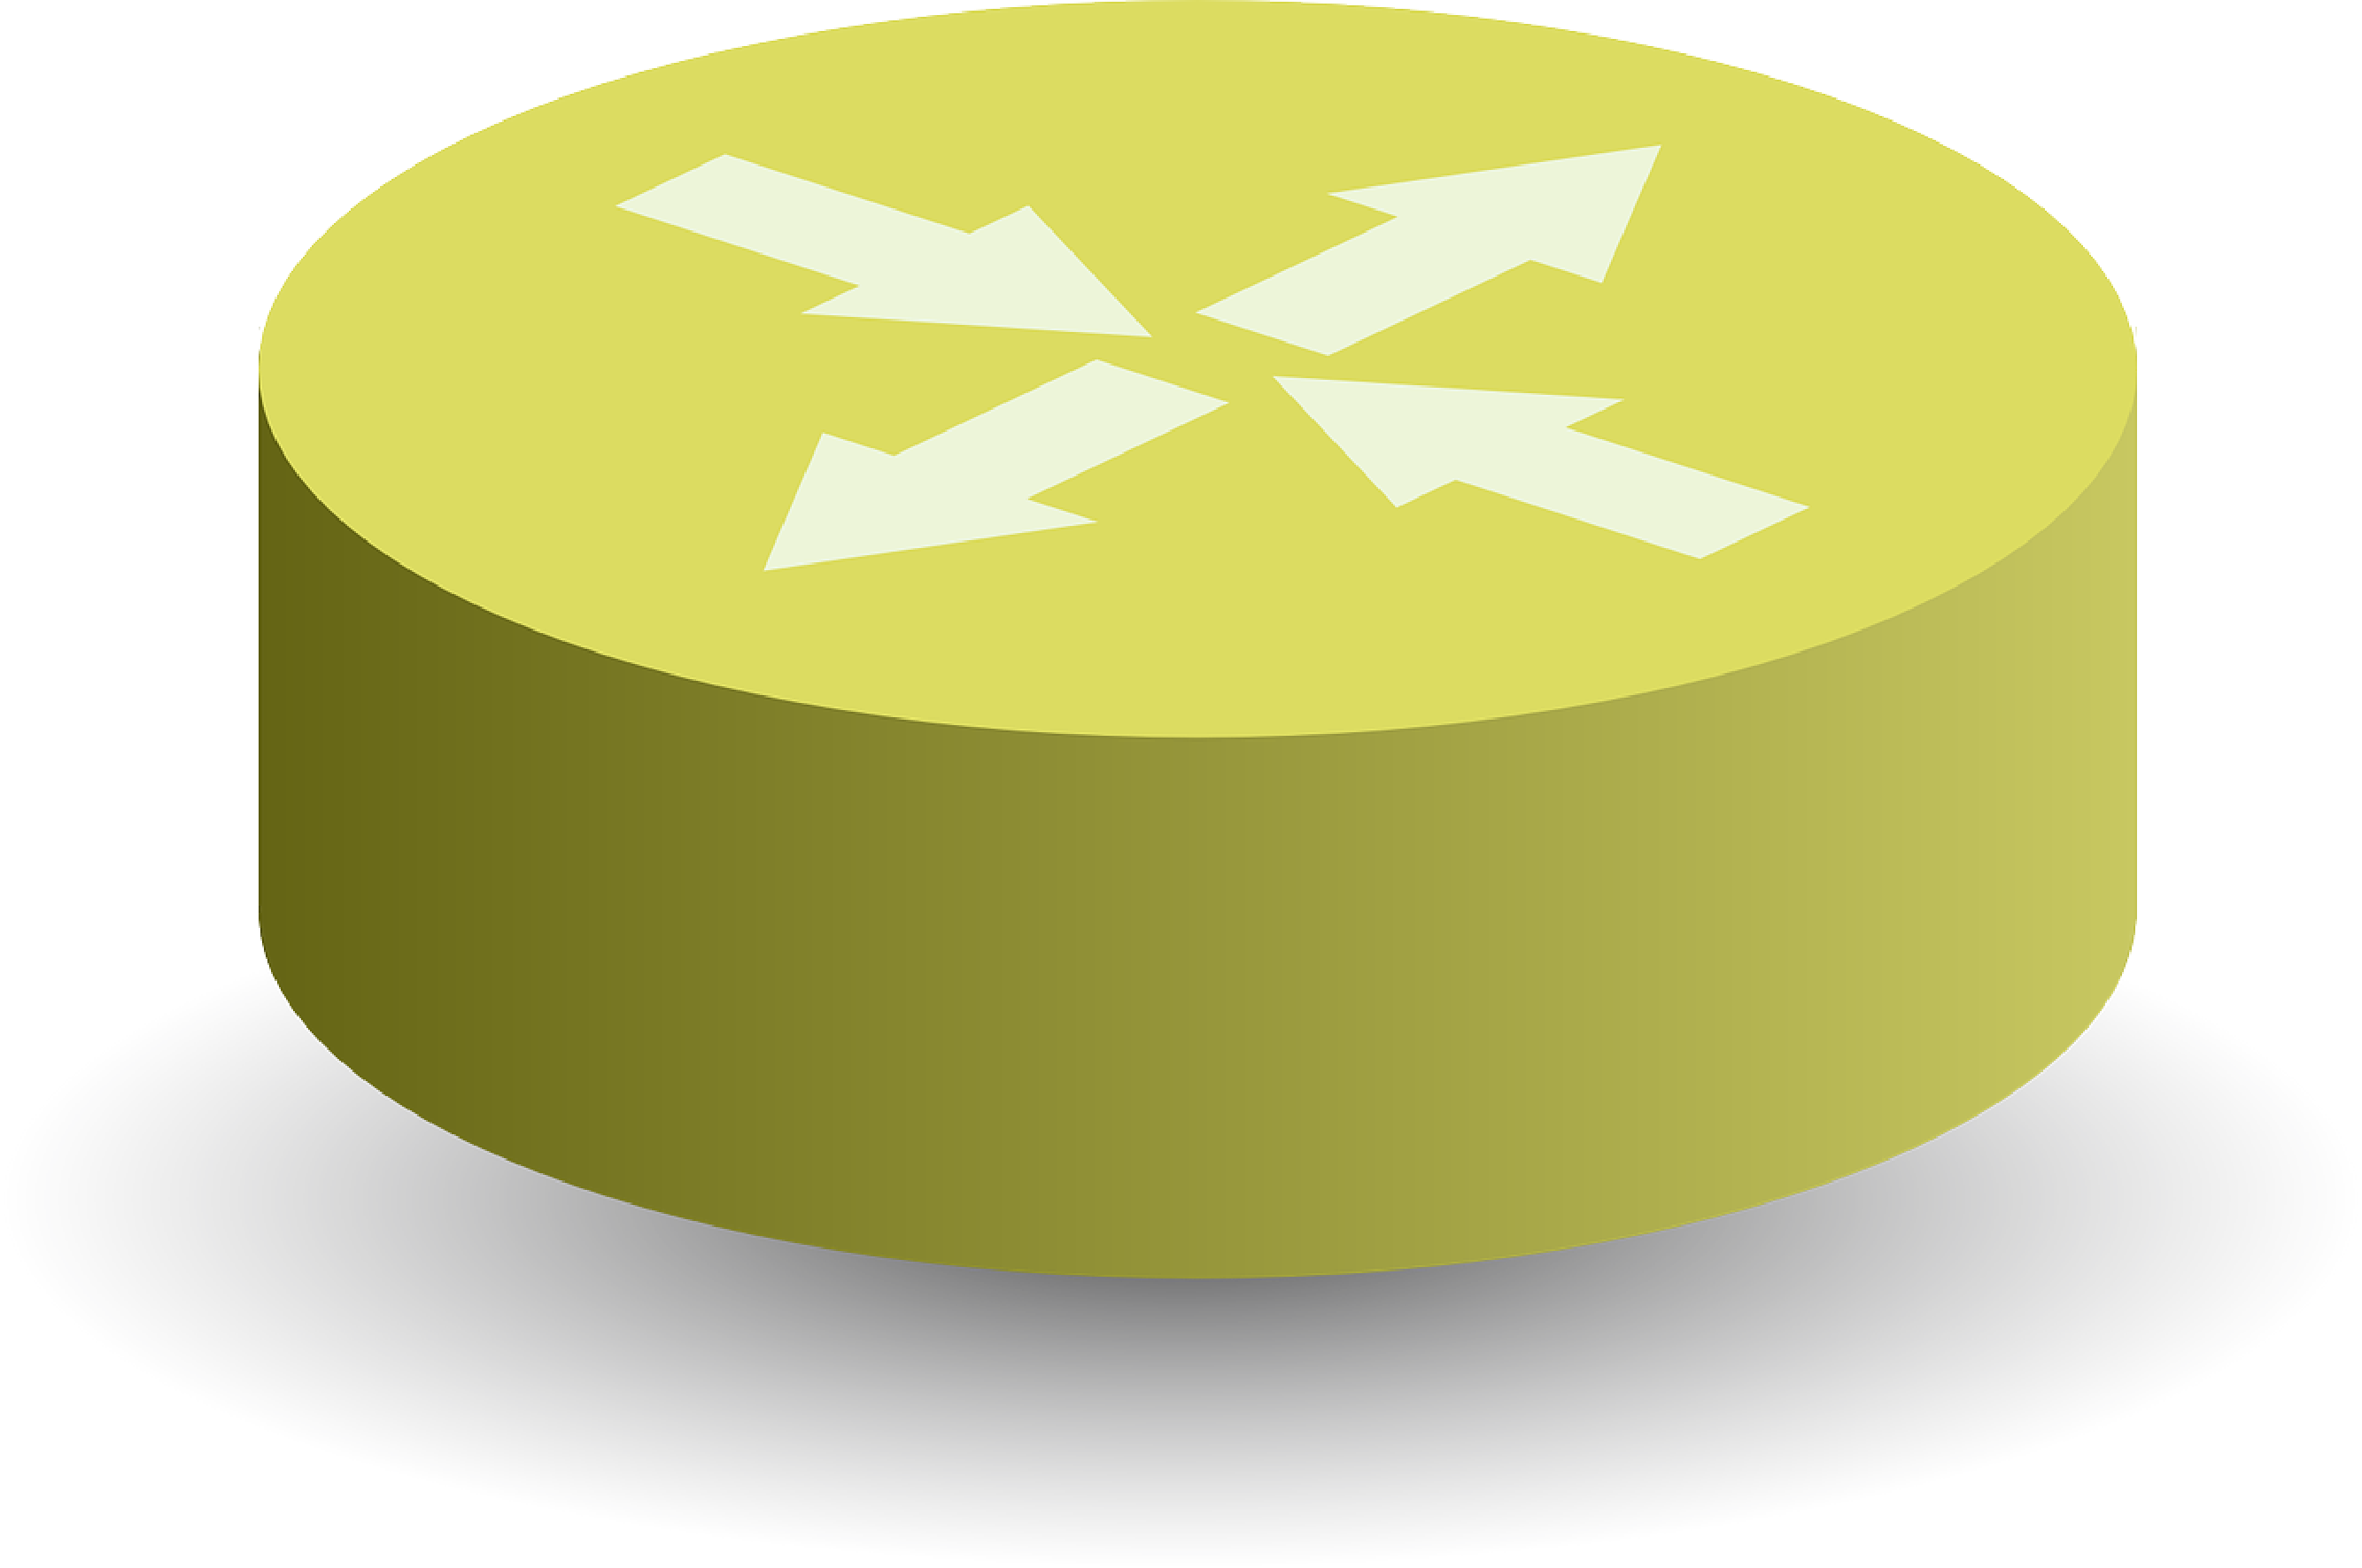
\includegraphics[width=52.5pt,height=52.5pt]{figures/router-158644_1280.pdf}};
%Image [id:dp9036637747838848] 
\draw (382.5,257.5) node  {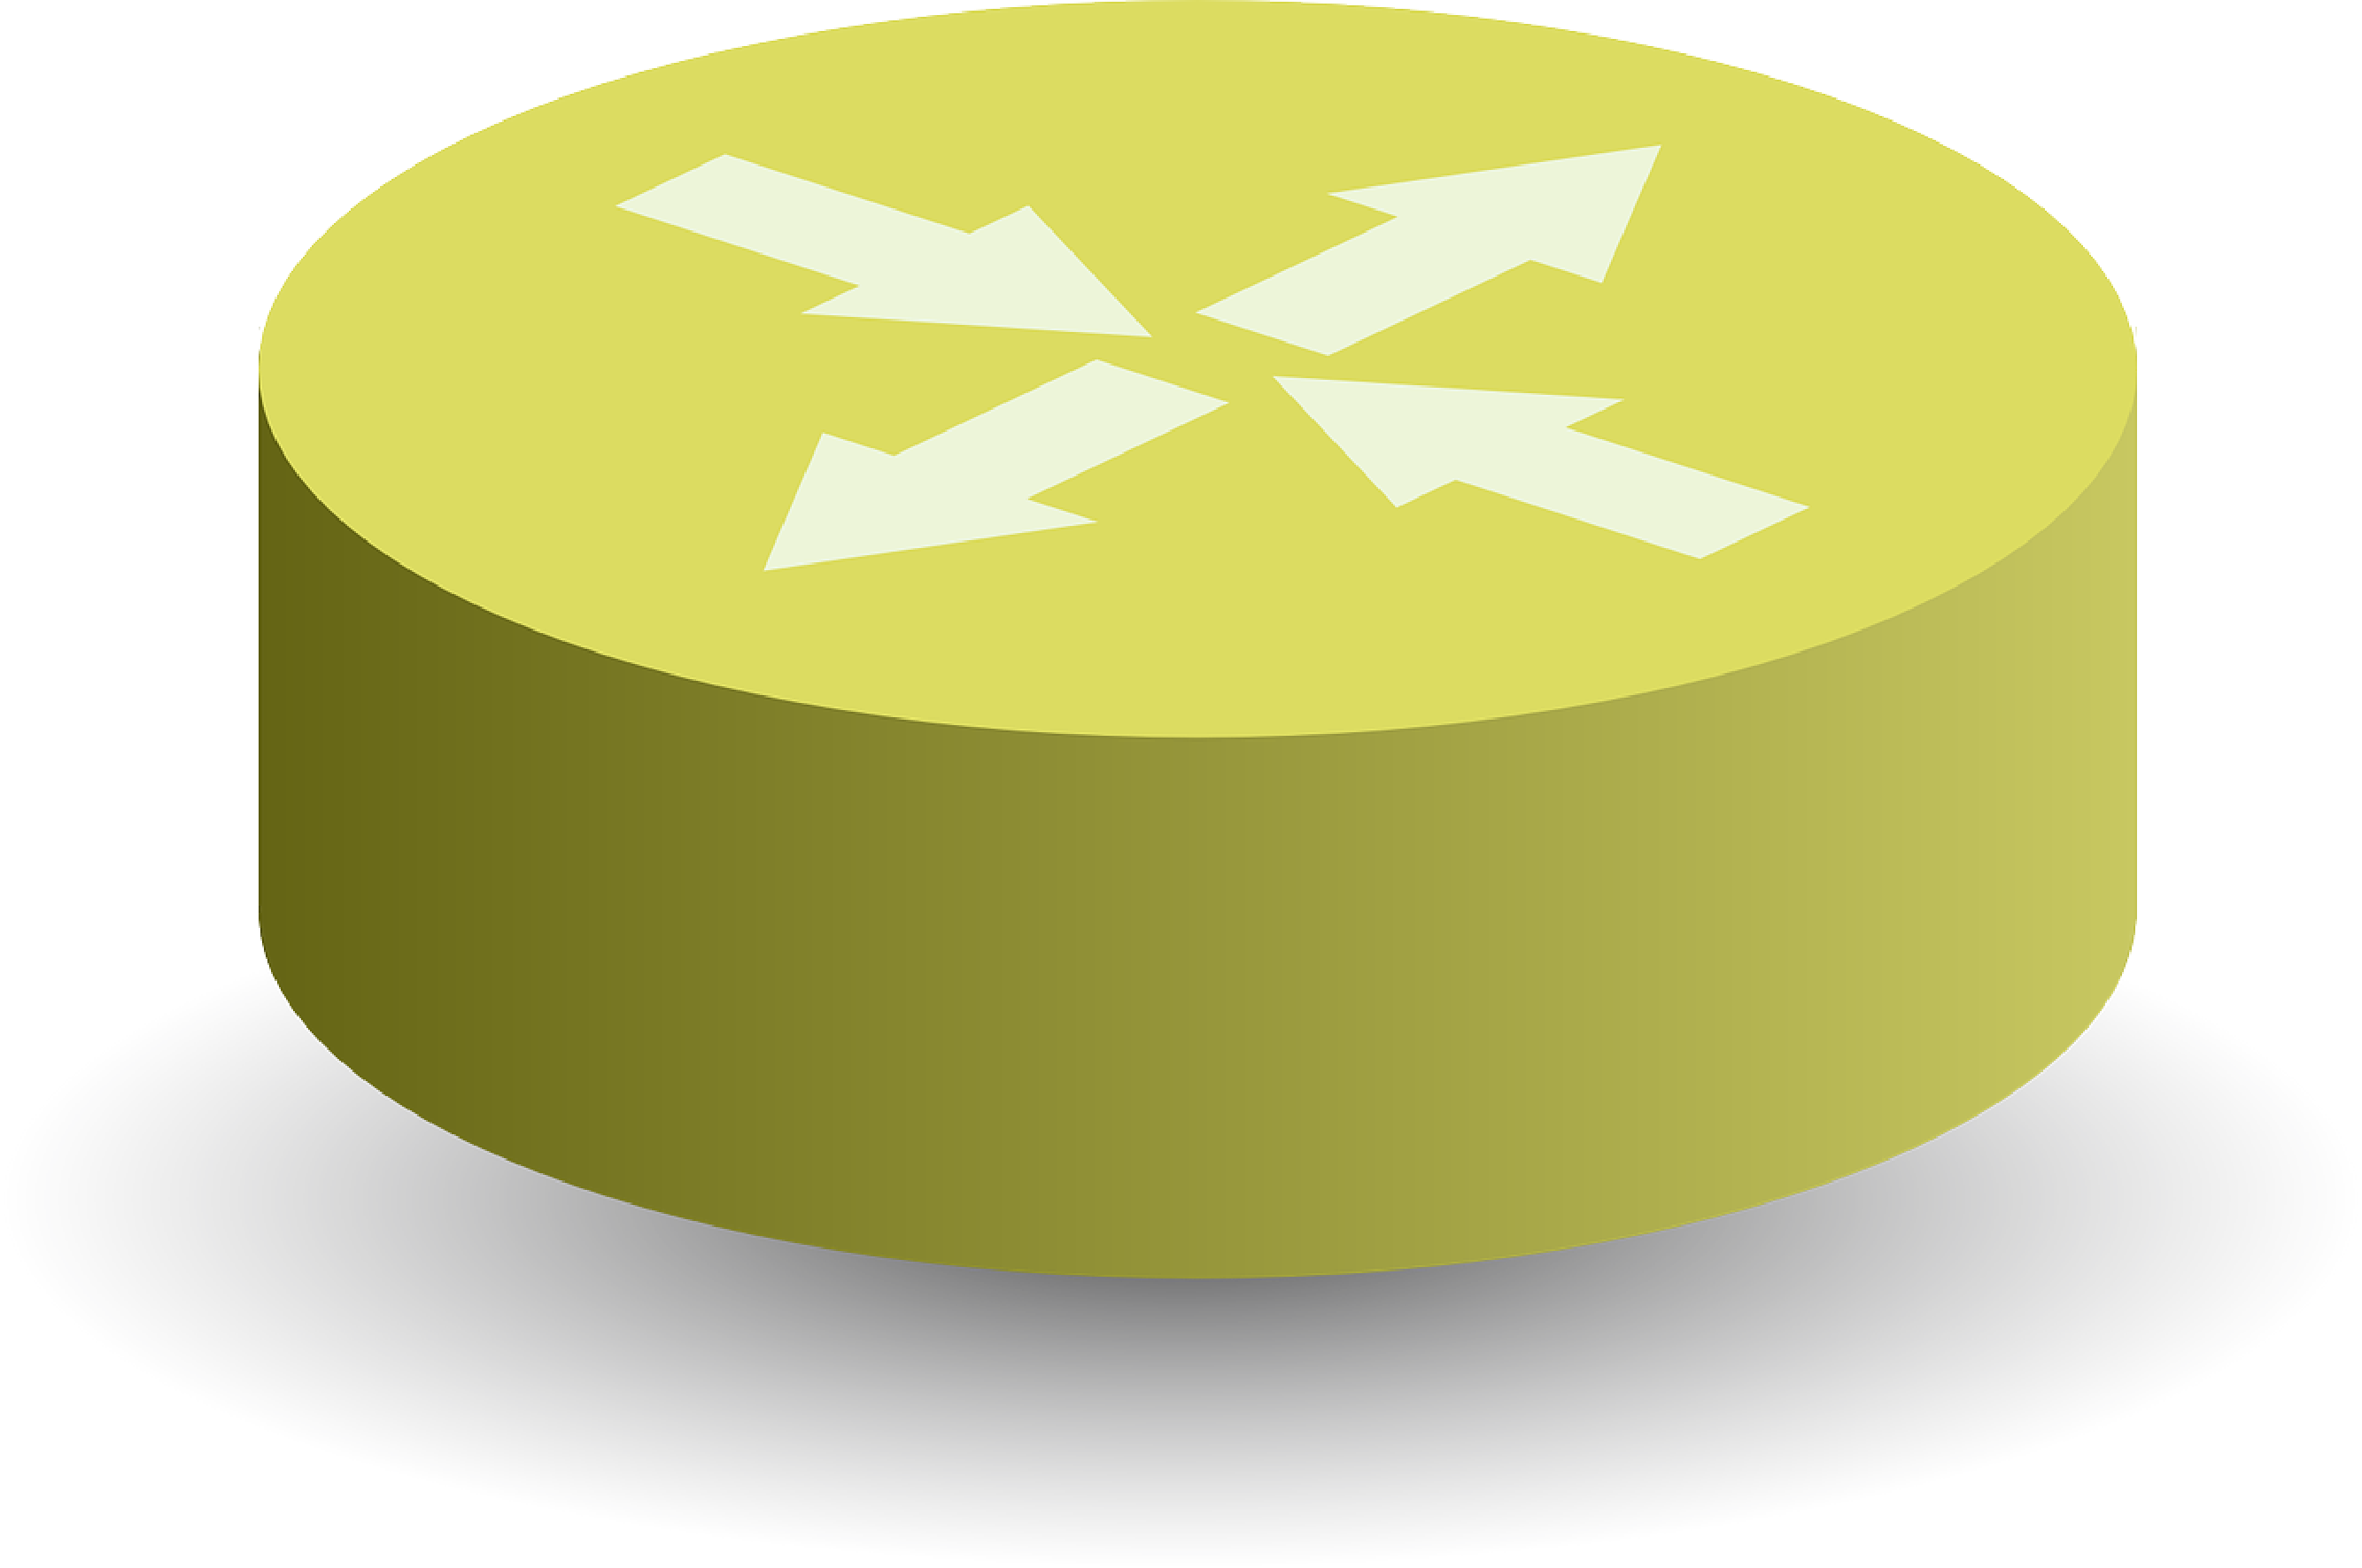
\includegraphics[width=52.5pt,height=52.5pt]{figures/router-158644_1280.pdf}};
%Image [id:dp5664602004547369] 
\draw (472,257.5) node  {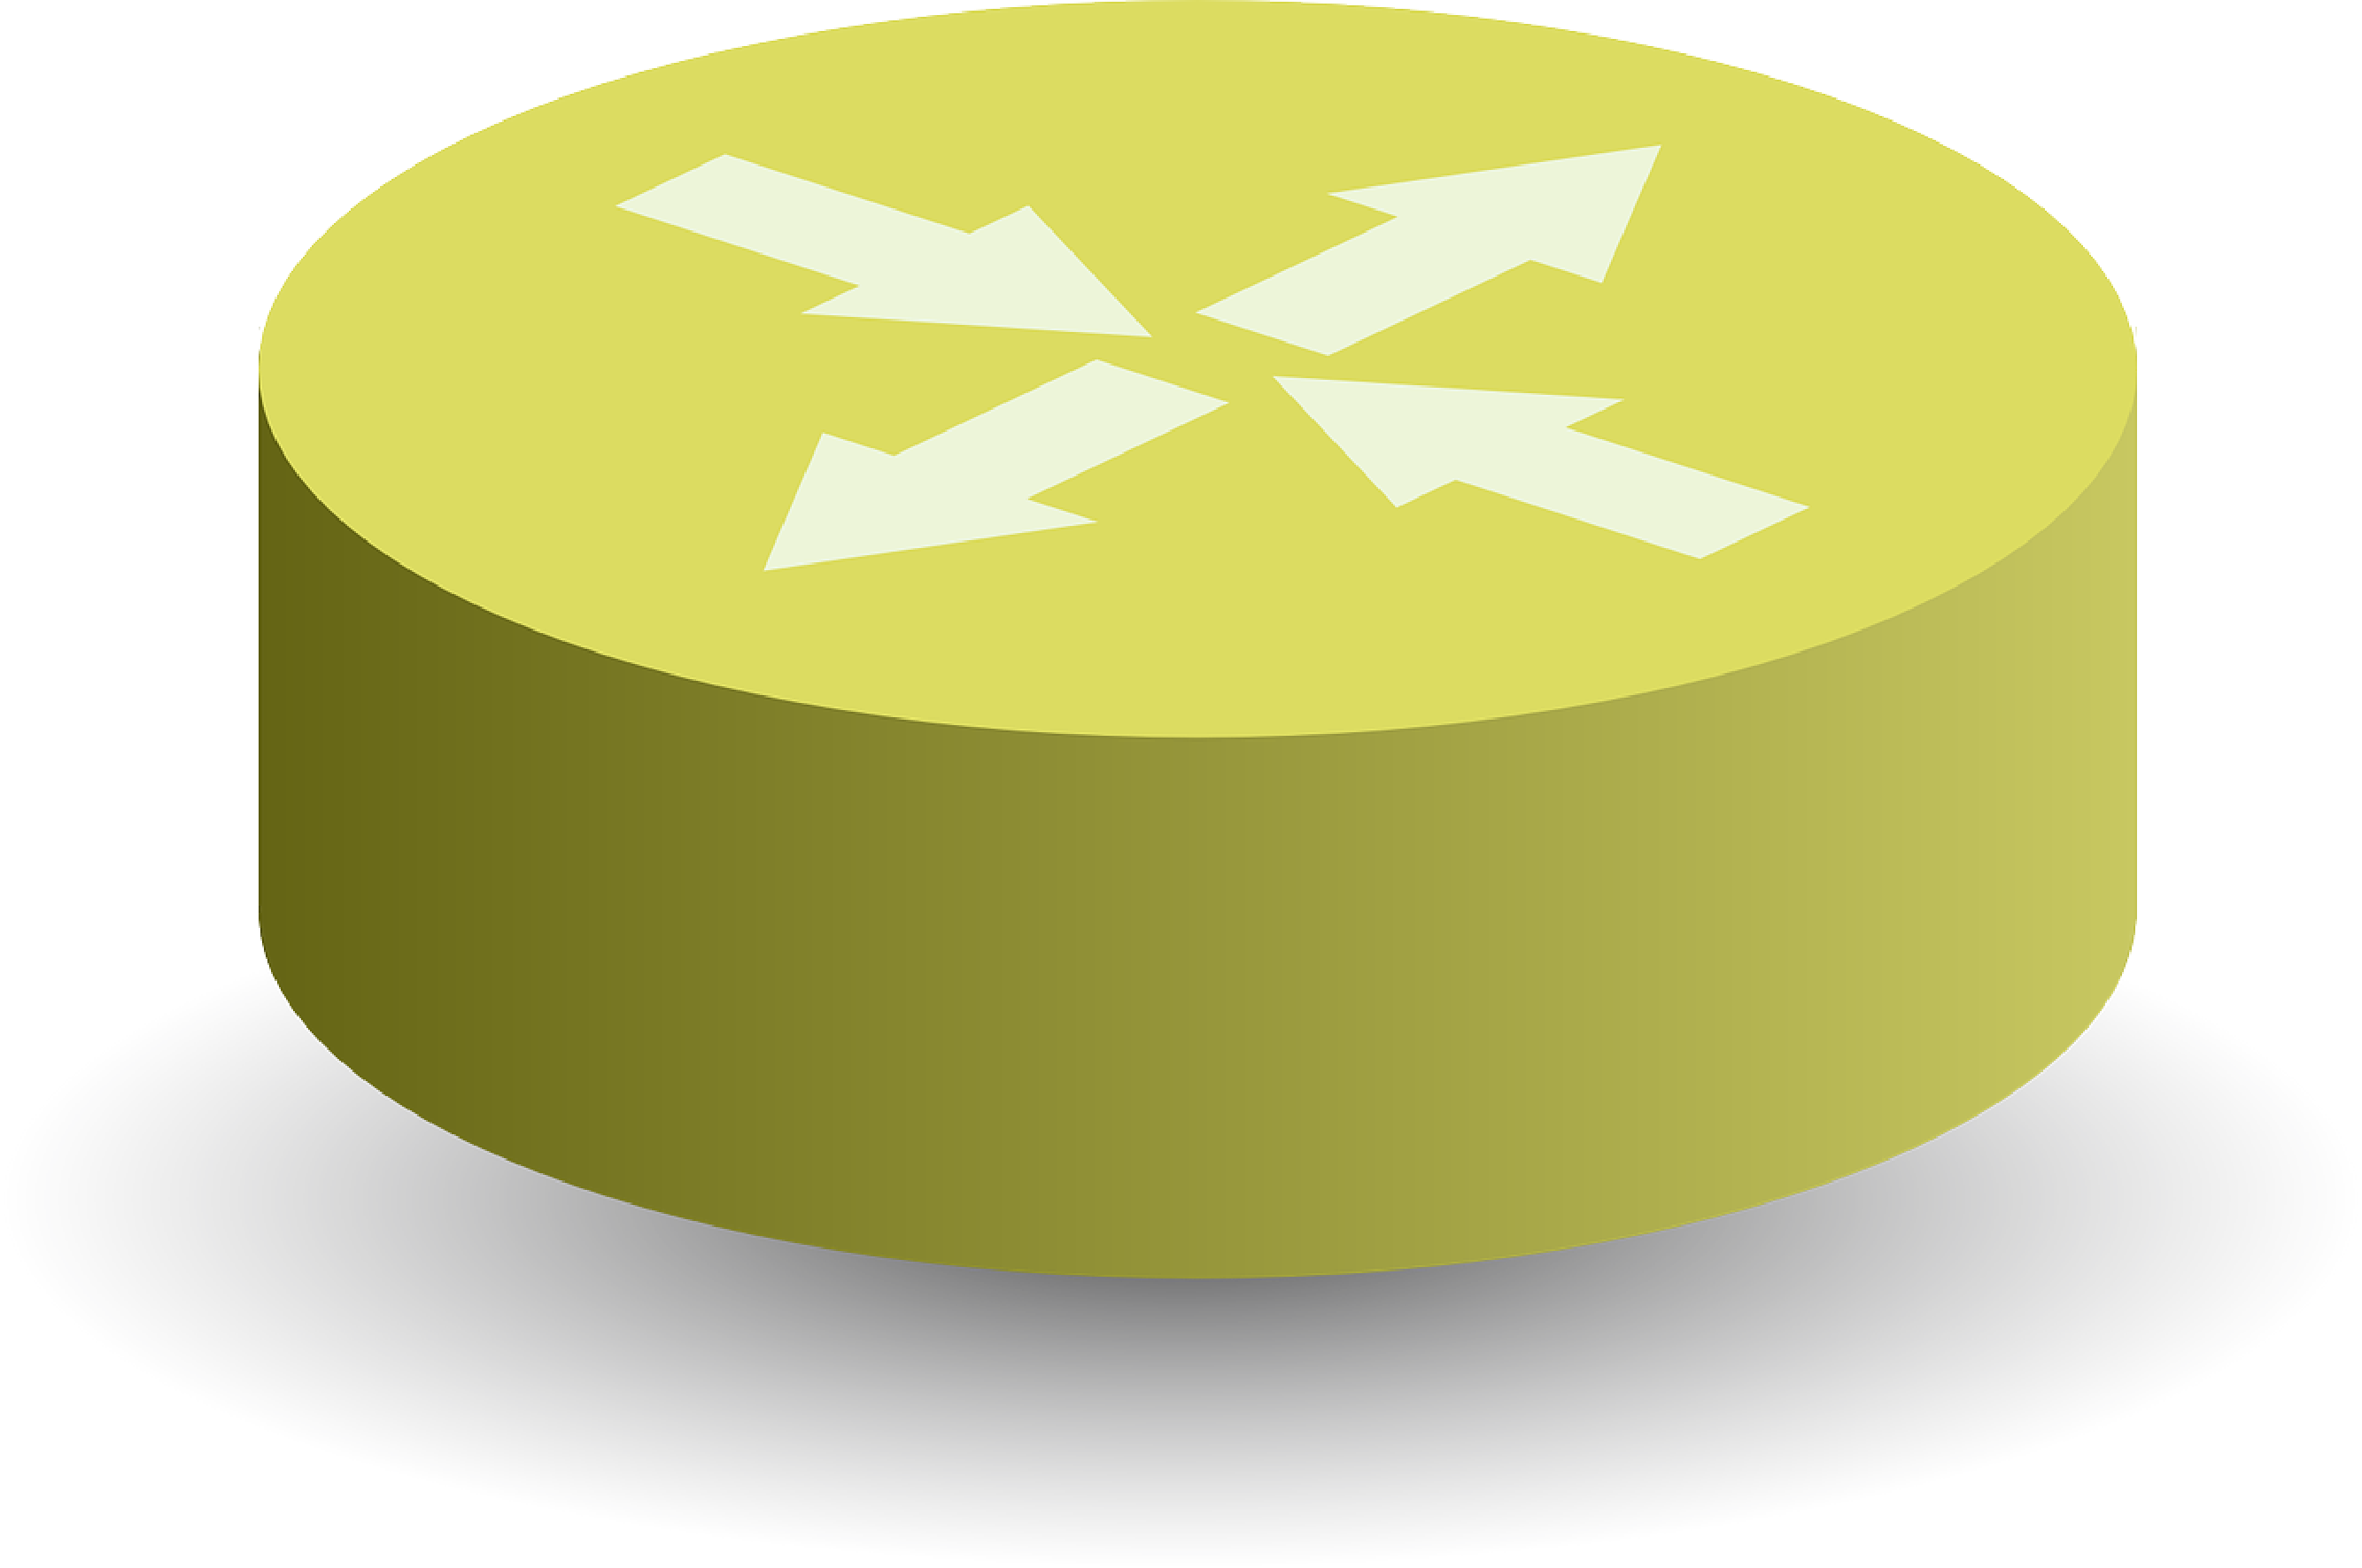
\includegraphics[width=52.5pt,height=52.5pt]{figures/router-158644_1280.pdf}};

%Rounded Rect [id:dp12210271864300348] 
\draw  [fill={rgb, 255:red, 255; green, 248; blue, 177 }  ,fill opacity=1 ] (26,177.73) .. controls (26,160.76) and (39.76,147) .. (56.73,147) -- (184.27,147) .. controls (201.24,147) and (215,160.76) .. (215,177.73) -- (215,269.93) .. controls (215,286.91) and (201.24,300.67) .. (184.27,300.67) -- (56.73,300.67) .. controls (39.76,300.67) and (26,286.91) .. (26,269.93) -- cycle ;
%Straight Lines [id:da9726012805844229] 
\draw    (56,209.67) -- (168,182) ;


%Image [id:dp05865651320982146] 
\draw (61,213.5) node  {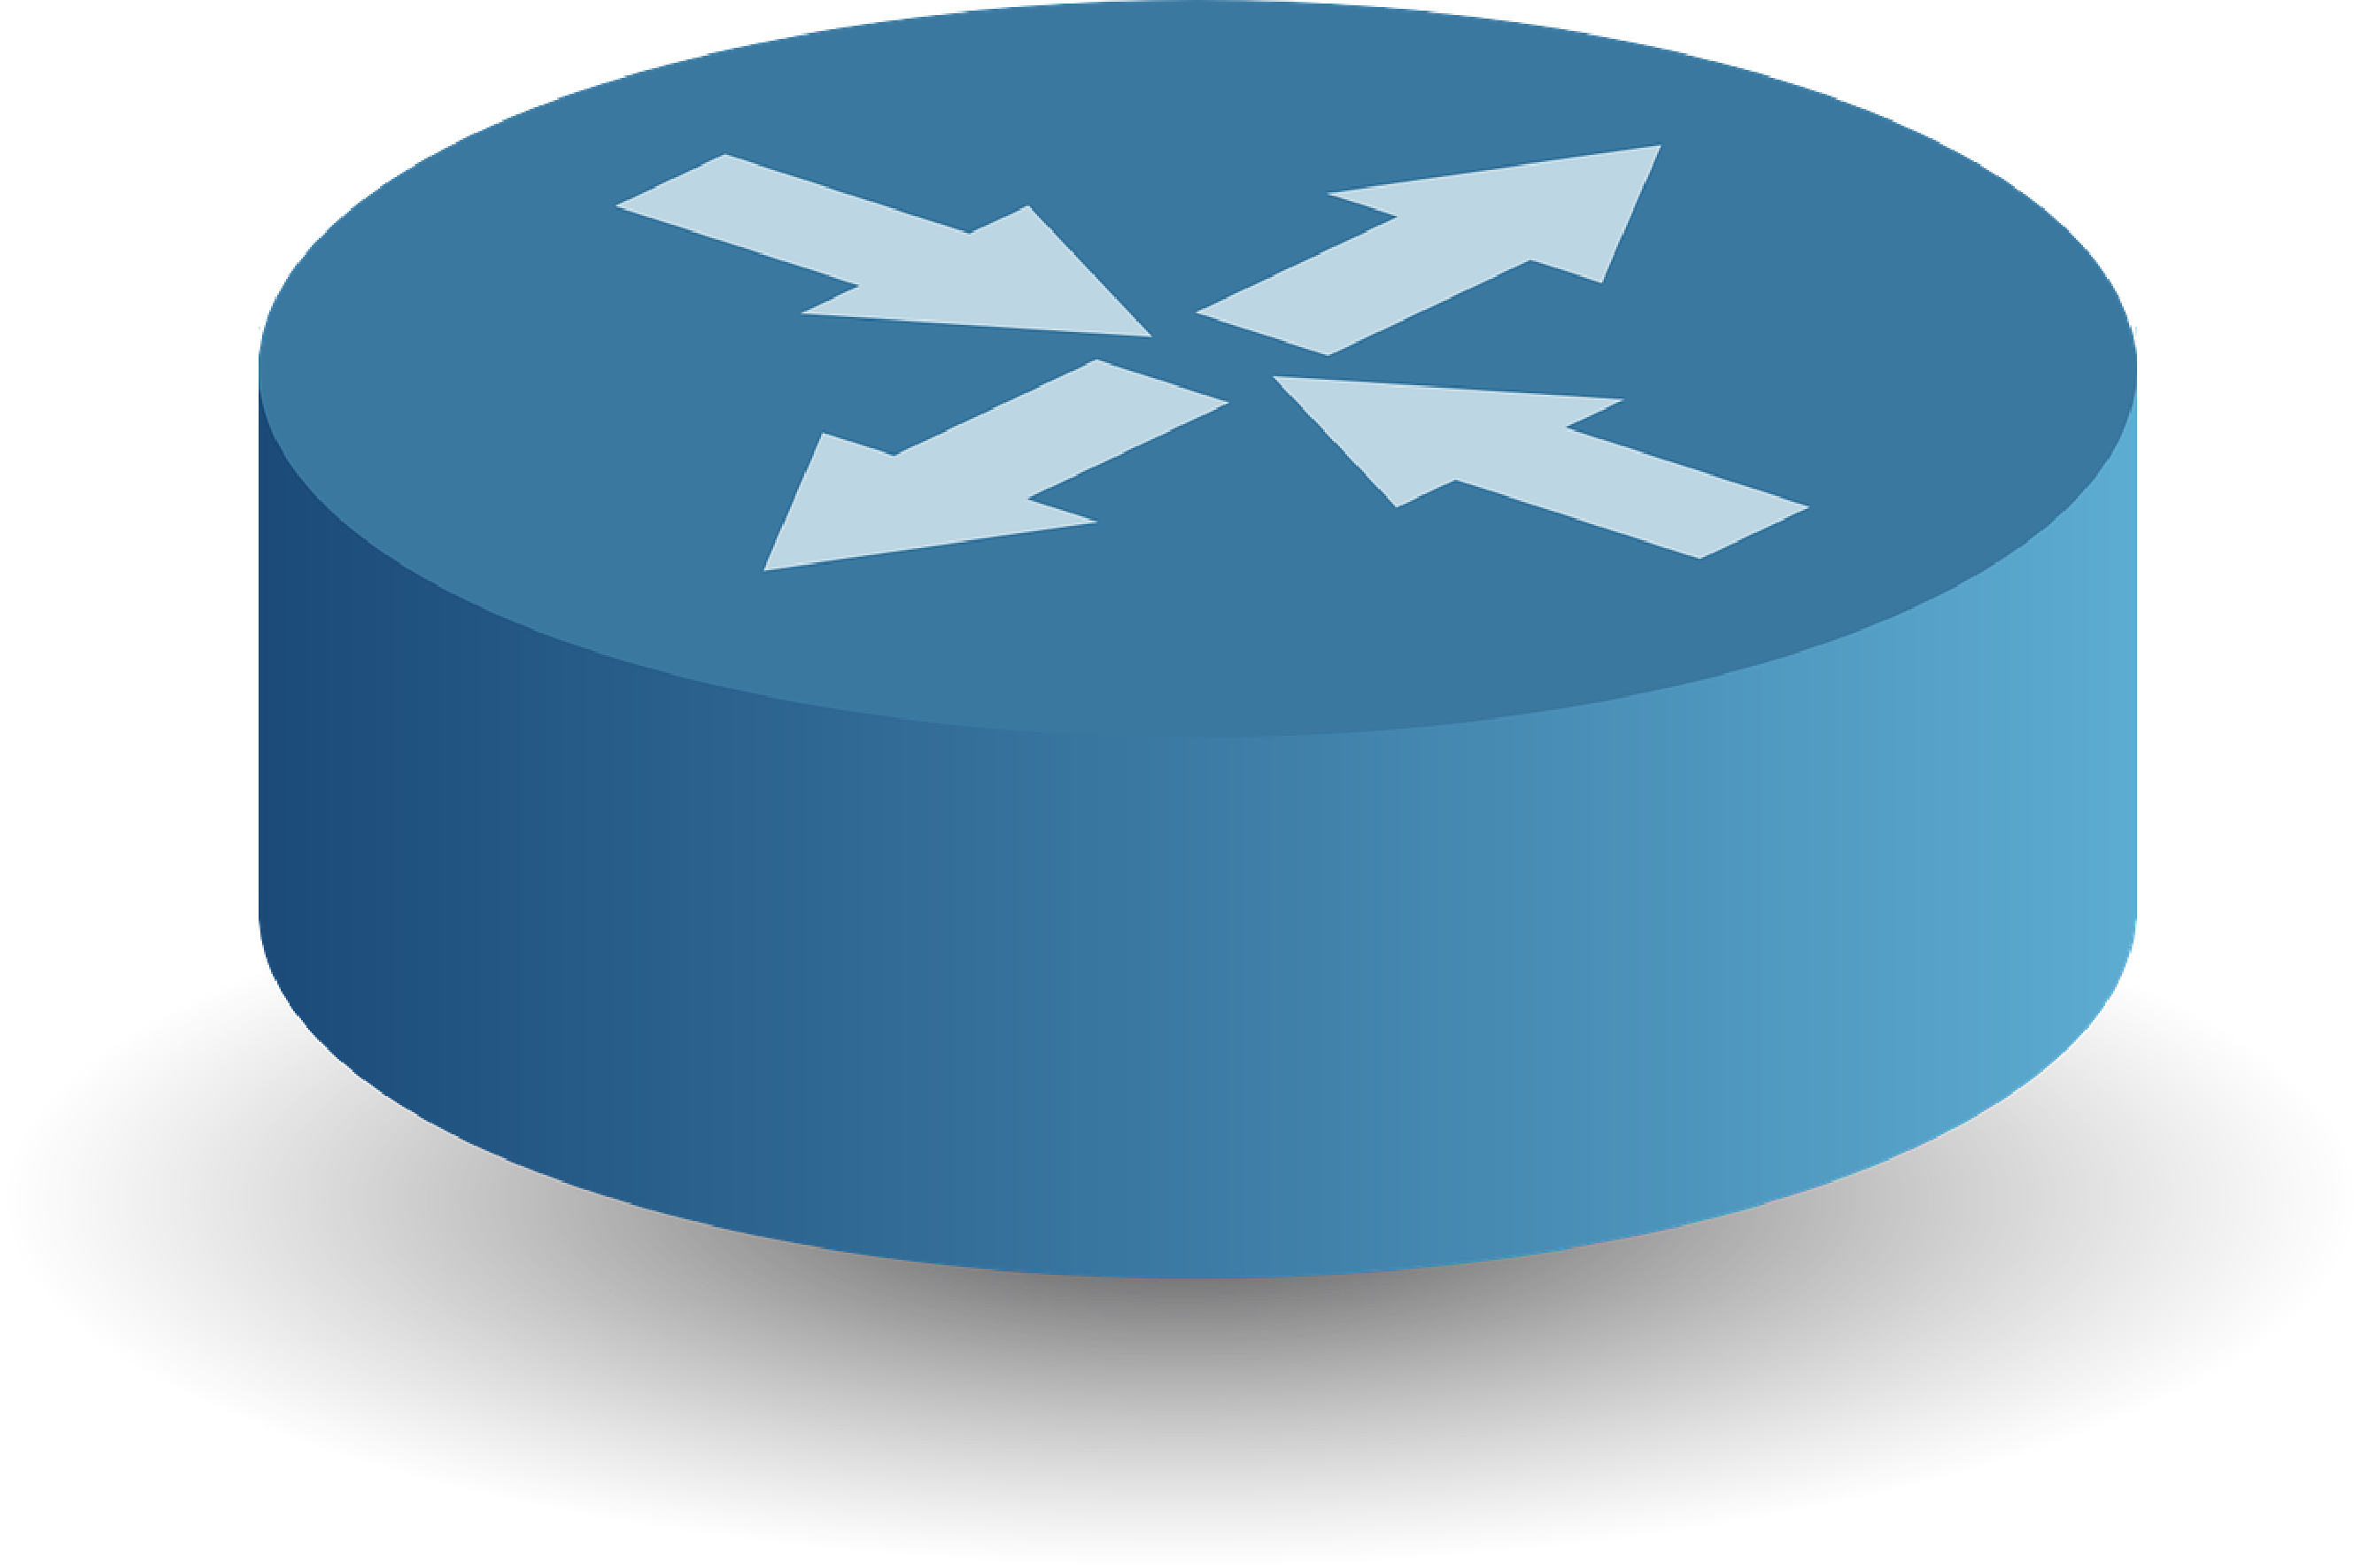
\includegraphics[width=52.5pt,height=52.5pt]{figures/router-29825_1280.pdf}};
%Image [id:dp21454722941873827] 
\draw (166,192.5) node  {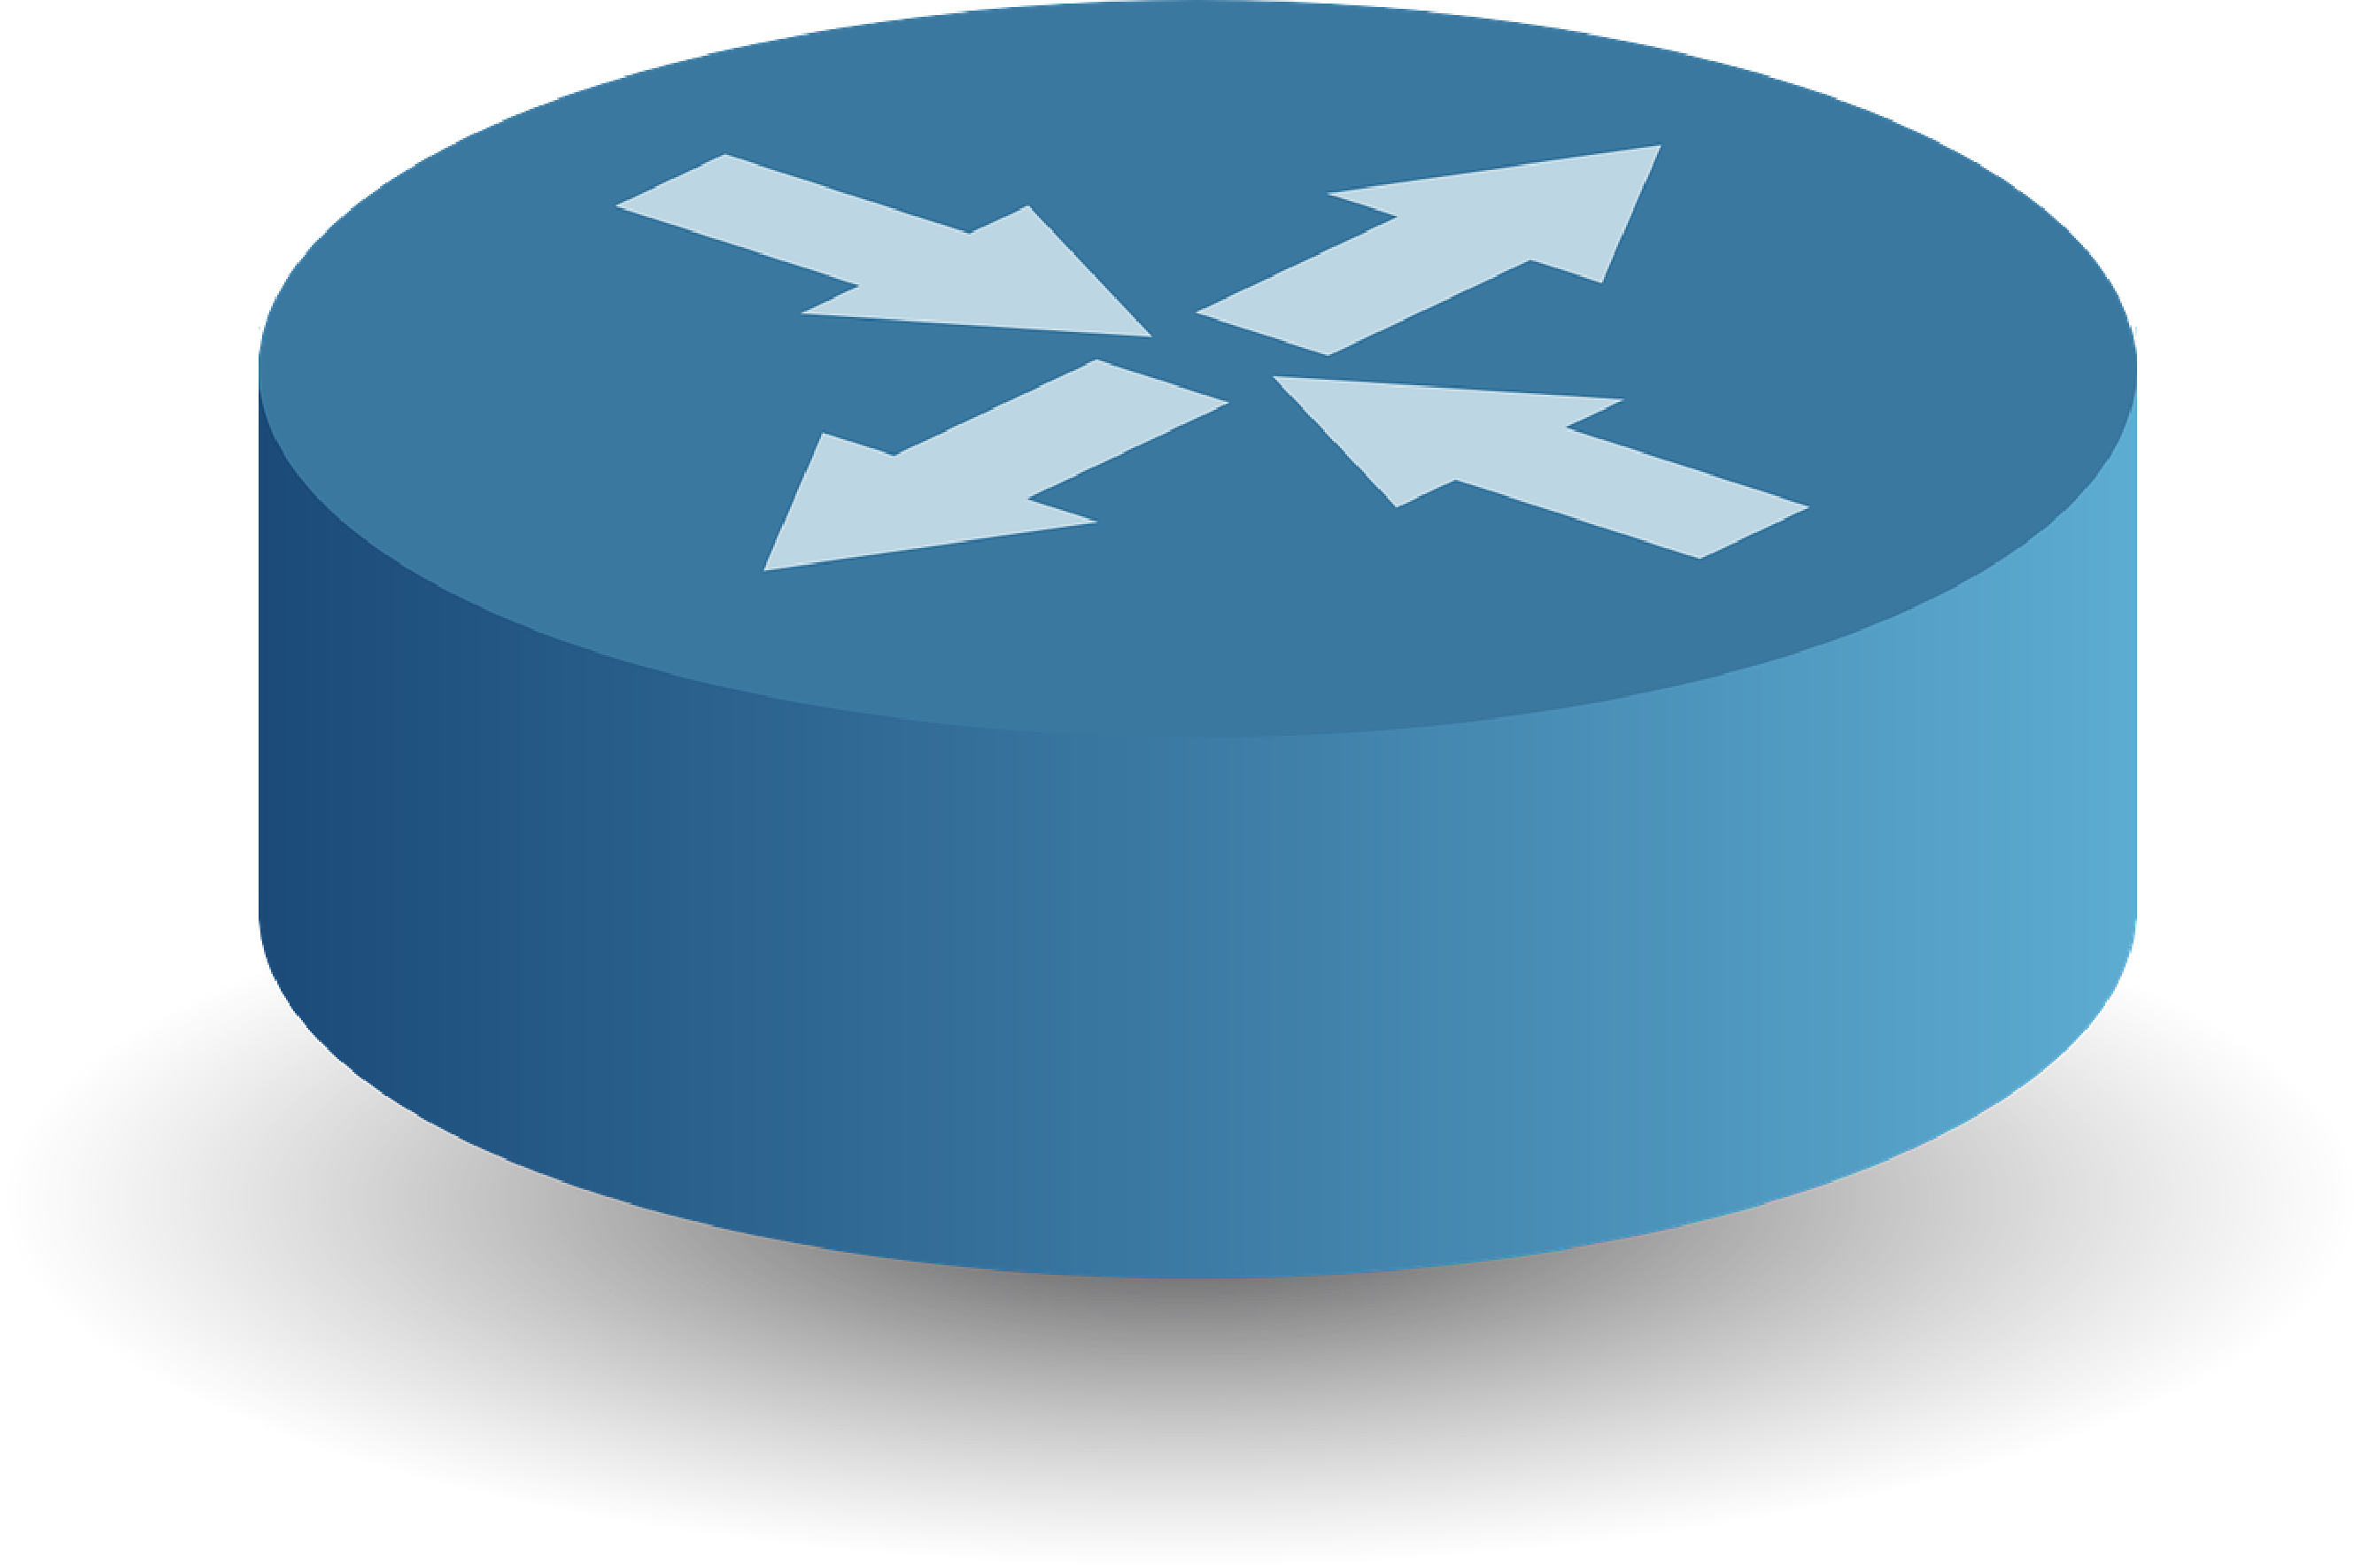
\includegraphics[width=52.5pt,height=52.5pt]{figures/router-29825_1280.pdf}};
%Straight Lines [id:da6563559723871784] 
\draw    (81,229.17) -- (138,254.67) ;


%Image [id:dp06912306094485043] 
\draw (136,267.5) node  {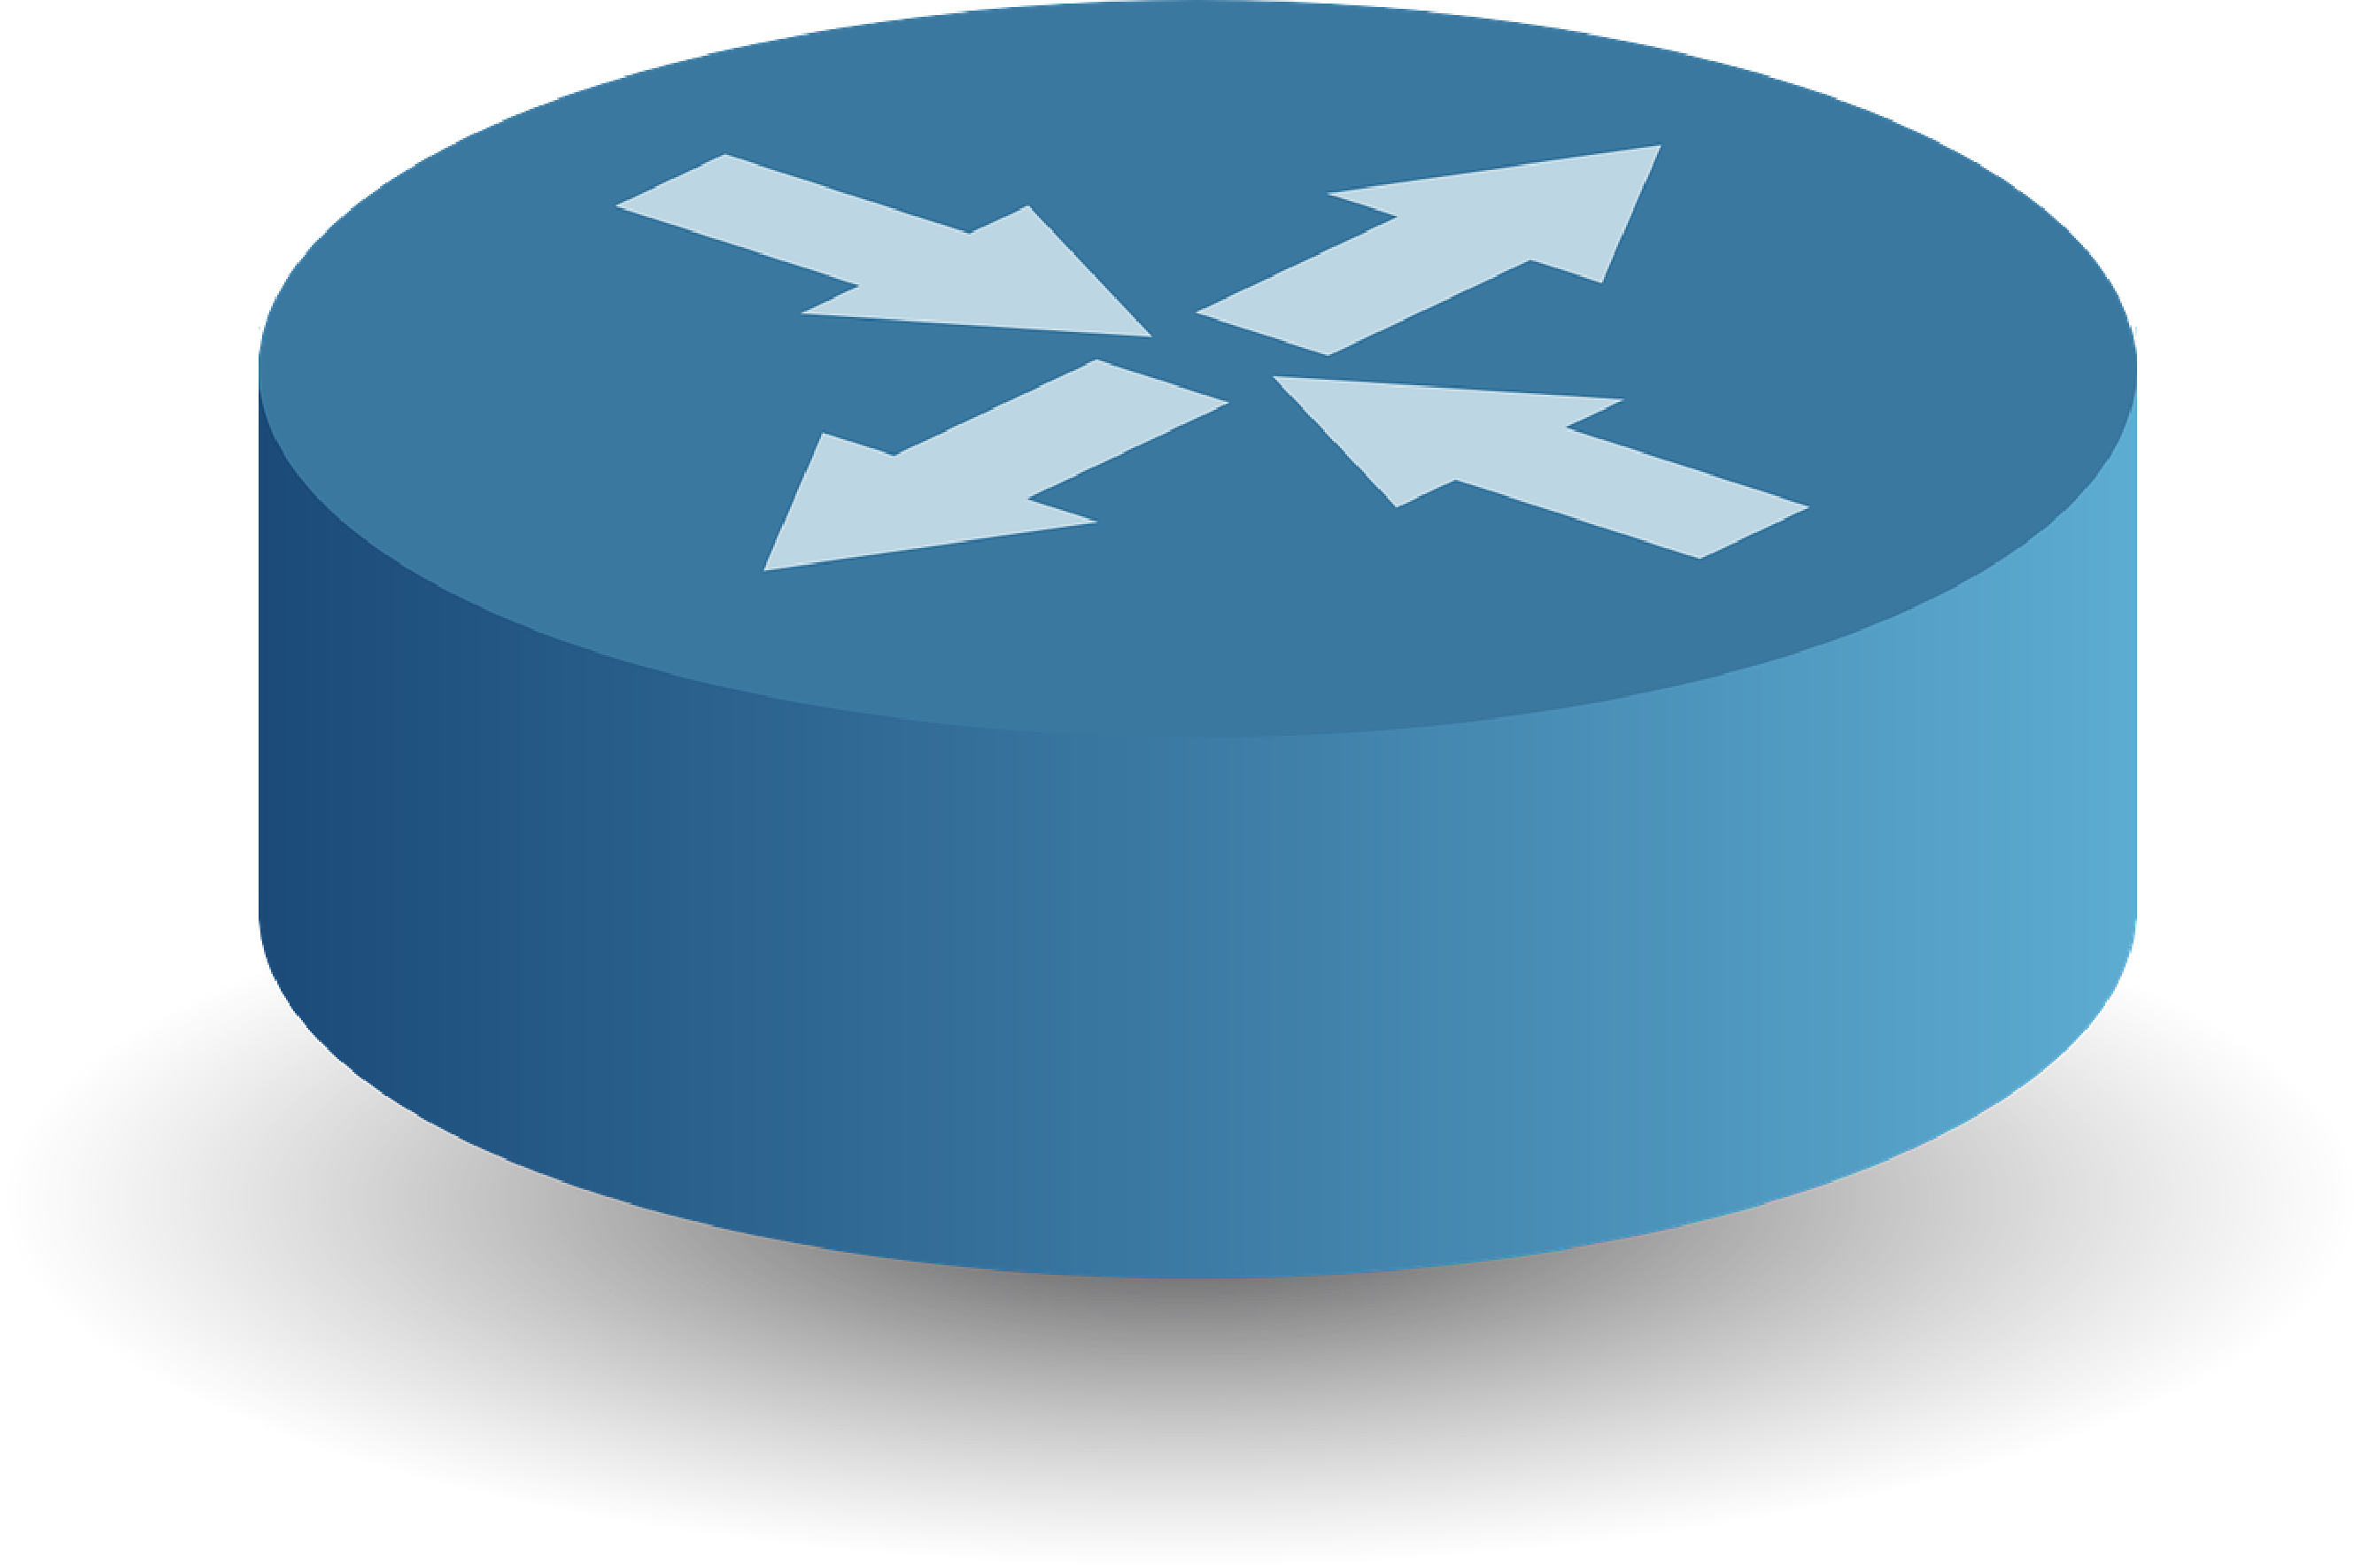
\includegraphics[width=52.5pt,height=52.5pt]{figures/router-29825_1280.pdf}};

%Rounded Rect [id:dp6027803870506079] 
\draw  [fill={rgb, 255:red, 184; green, 233; blue, 134 }  ,fill opacity=1 ] (26,398.47) .. controls (26,383.11) and (38.45,370.67) .. (53.8,370.67) -- (485.2,370.67) .. controls (500.55,370.67) and (513,383.11) .. (513,398.47) -- (513,481.87) .. controls (513,497.22) and (500.55,509.67) .. (485.2,509.67) -- (53.8,509.67) .. controls (38.45,509.67) and (26,497.22) .. (26,481.87) -- cycle ;
%Straight Lines [id:da6945688507769169] 
\draw    (79,428.67) -- (214,401.67) ;


%Straight Lines [id:da7153097807277008] 
\draw    (80,443.67) -- (171,466.67) ;


%Straight Lines [id:da07146248132512234] 
\draw    (174,473.67) -- (305,425) ;


%Straight Lines [id:da712168358630716] 
\draw    (214,401.67) -- (315,422) ;


%Straight Lines [id:da3878023367119837] 
\draw    (312,430) -- (465,415) ;


%Straight Lines [id:da7341038378459249] 
\draw    (321,430) -- (477,476.67) ;


%Image [id:dp11940314744085934] 
\draw (70,443.5) node  {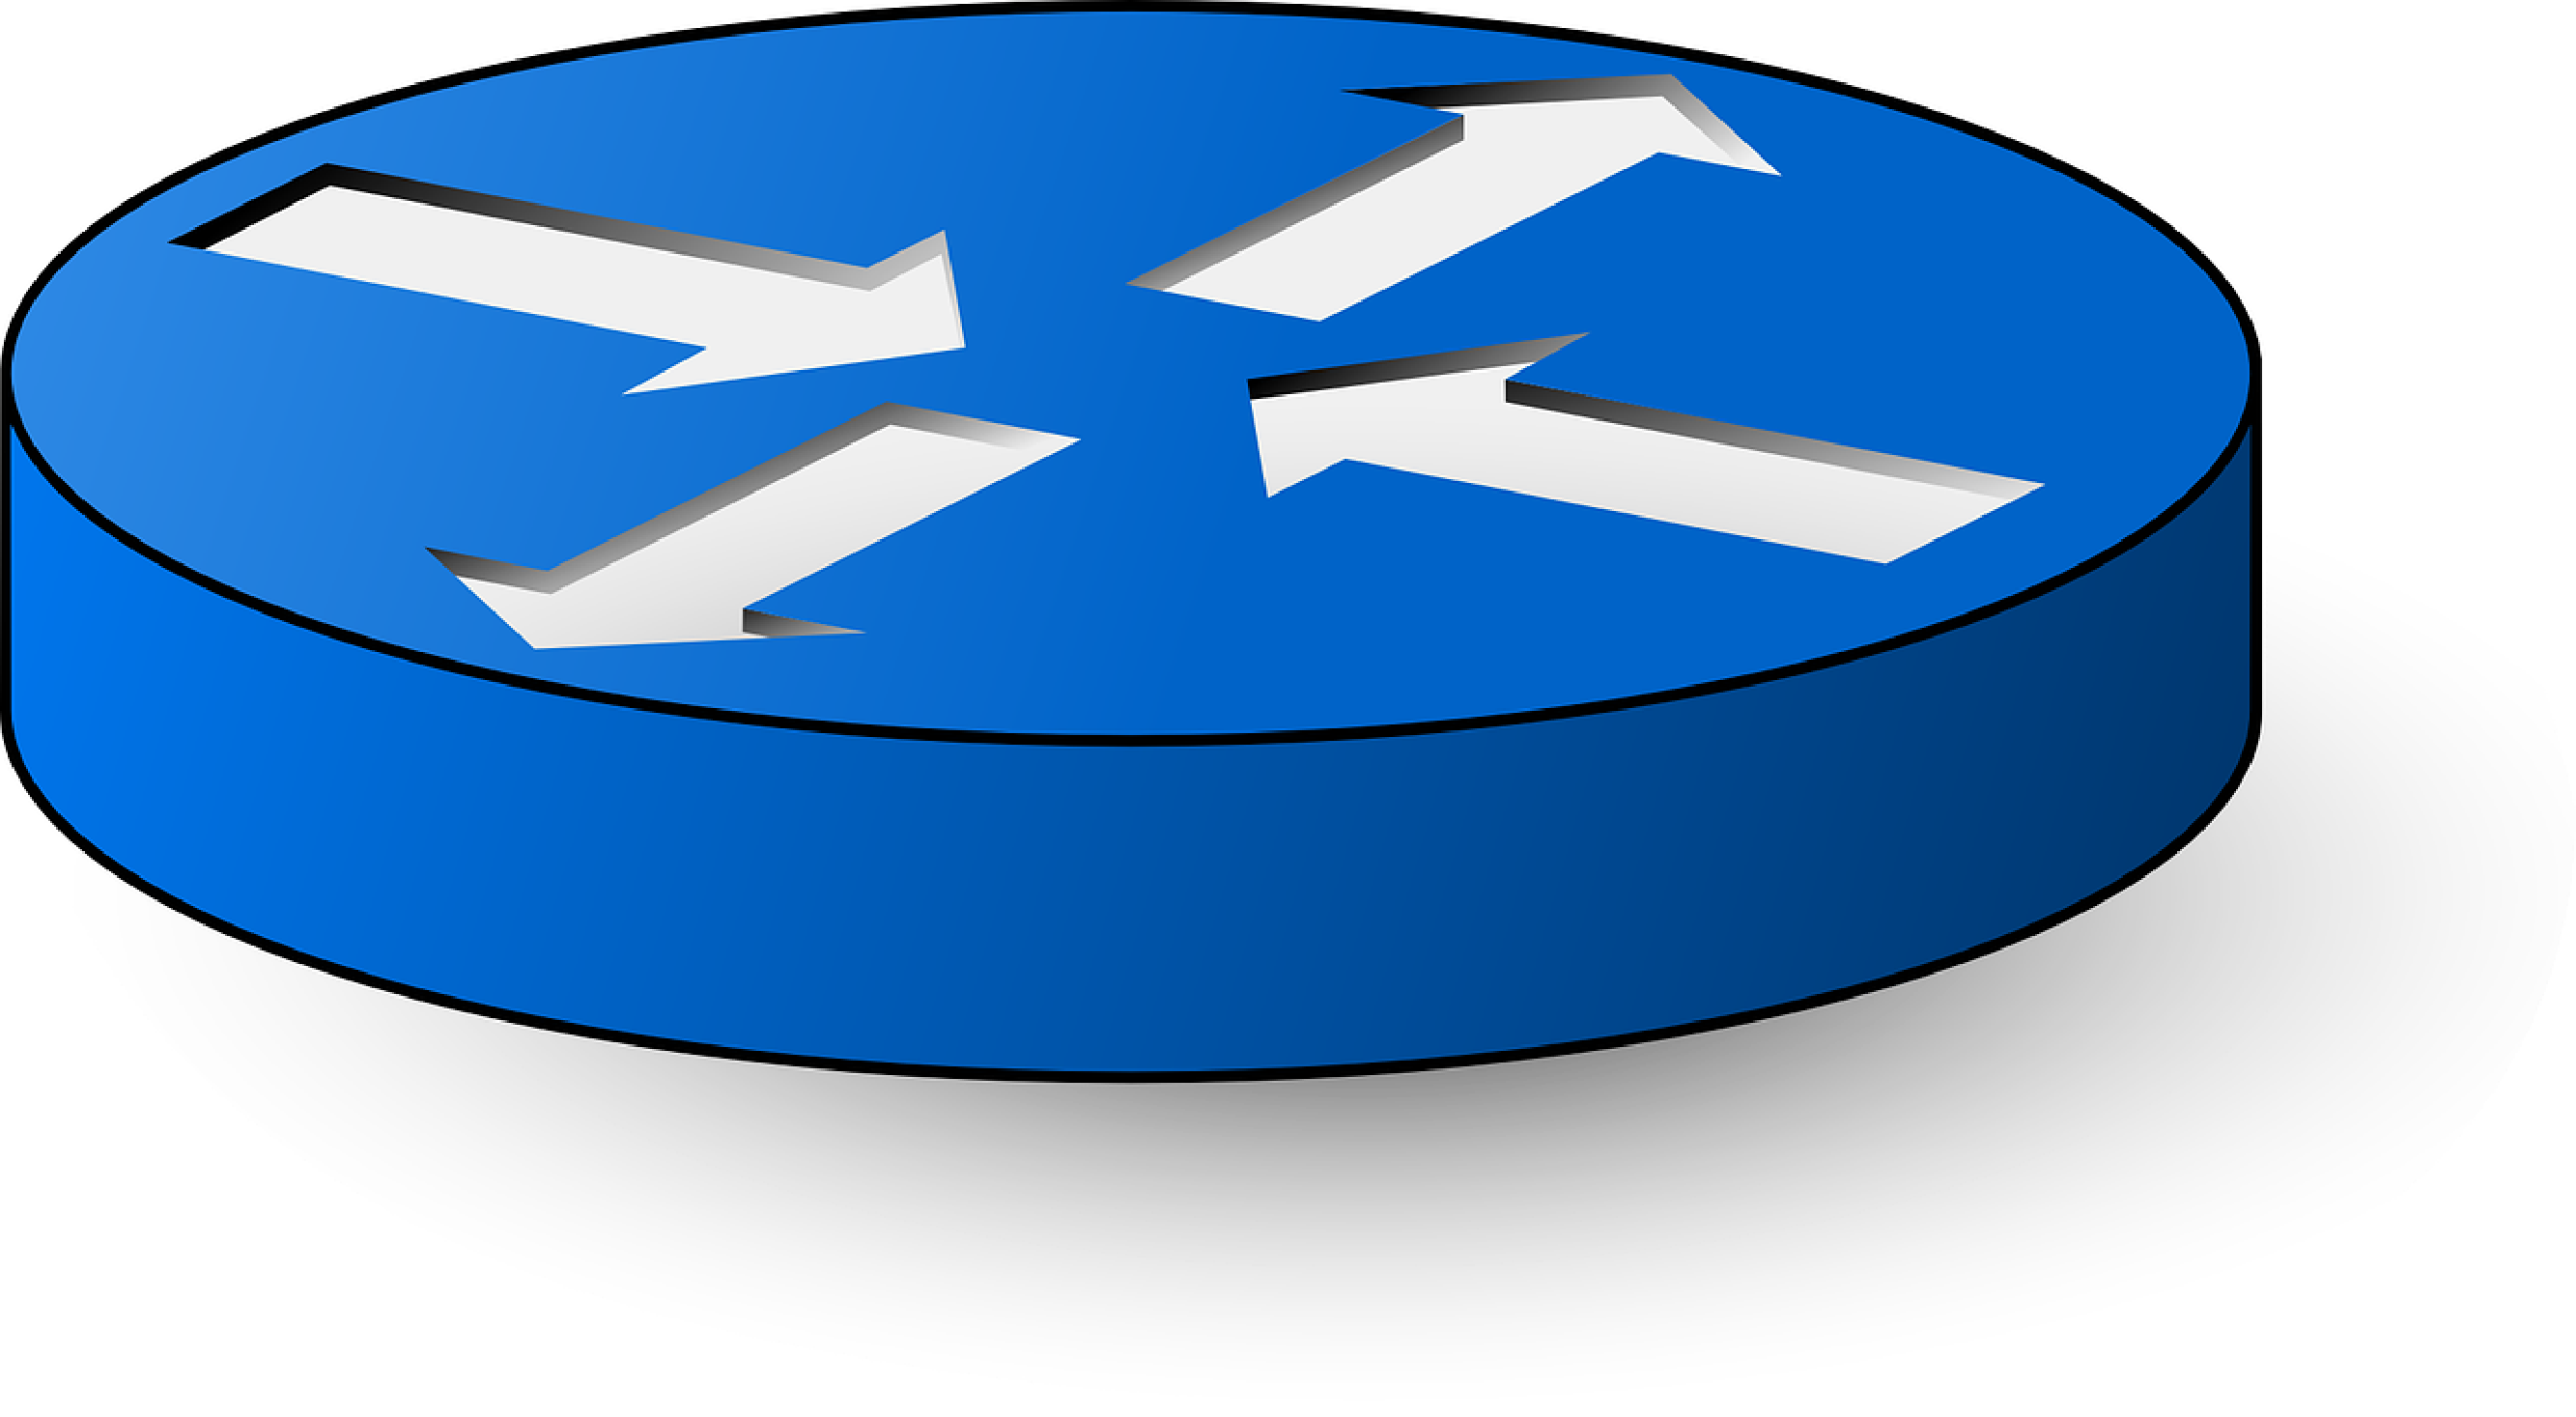
\includegraphics[width=52.5pt,height=52.5pt]{figures/router-30140_1280.pdf}};
%Image [id:dp8117021899058734] 
\draw (160,474.5) node  {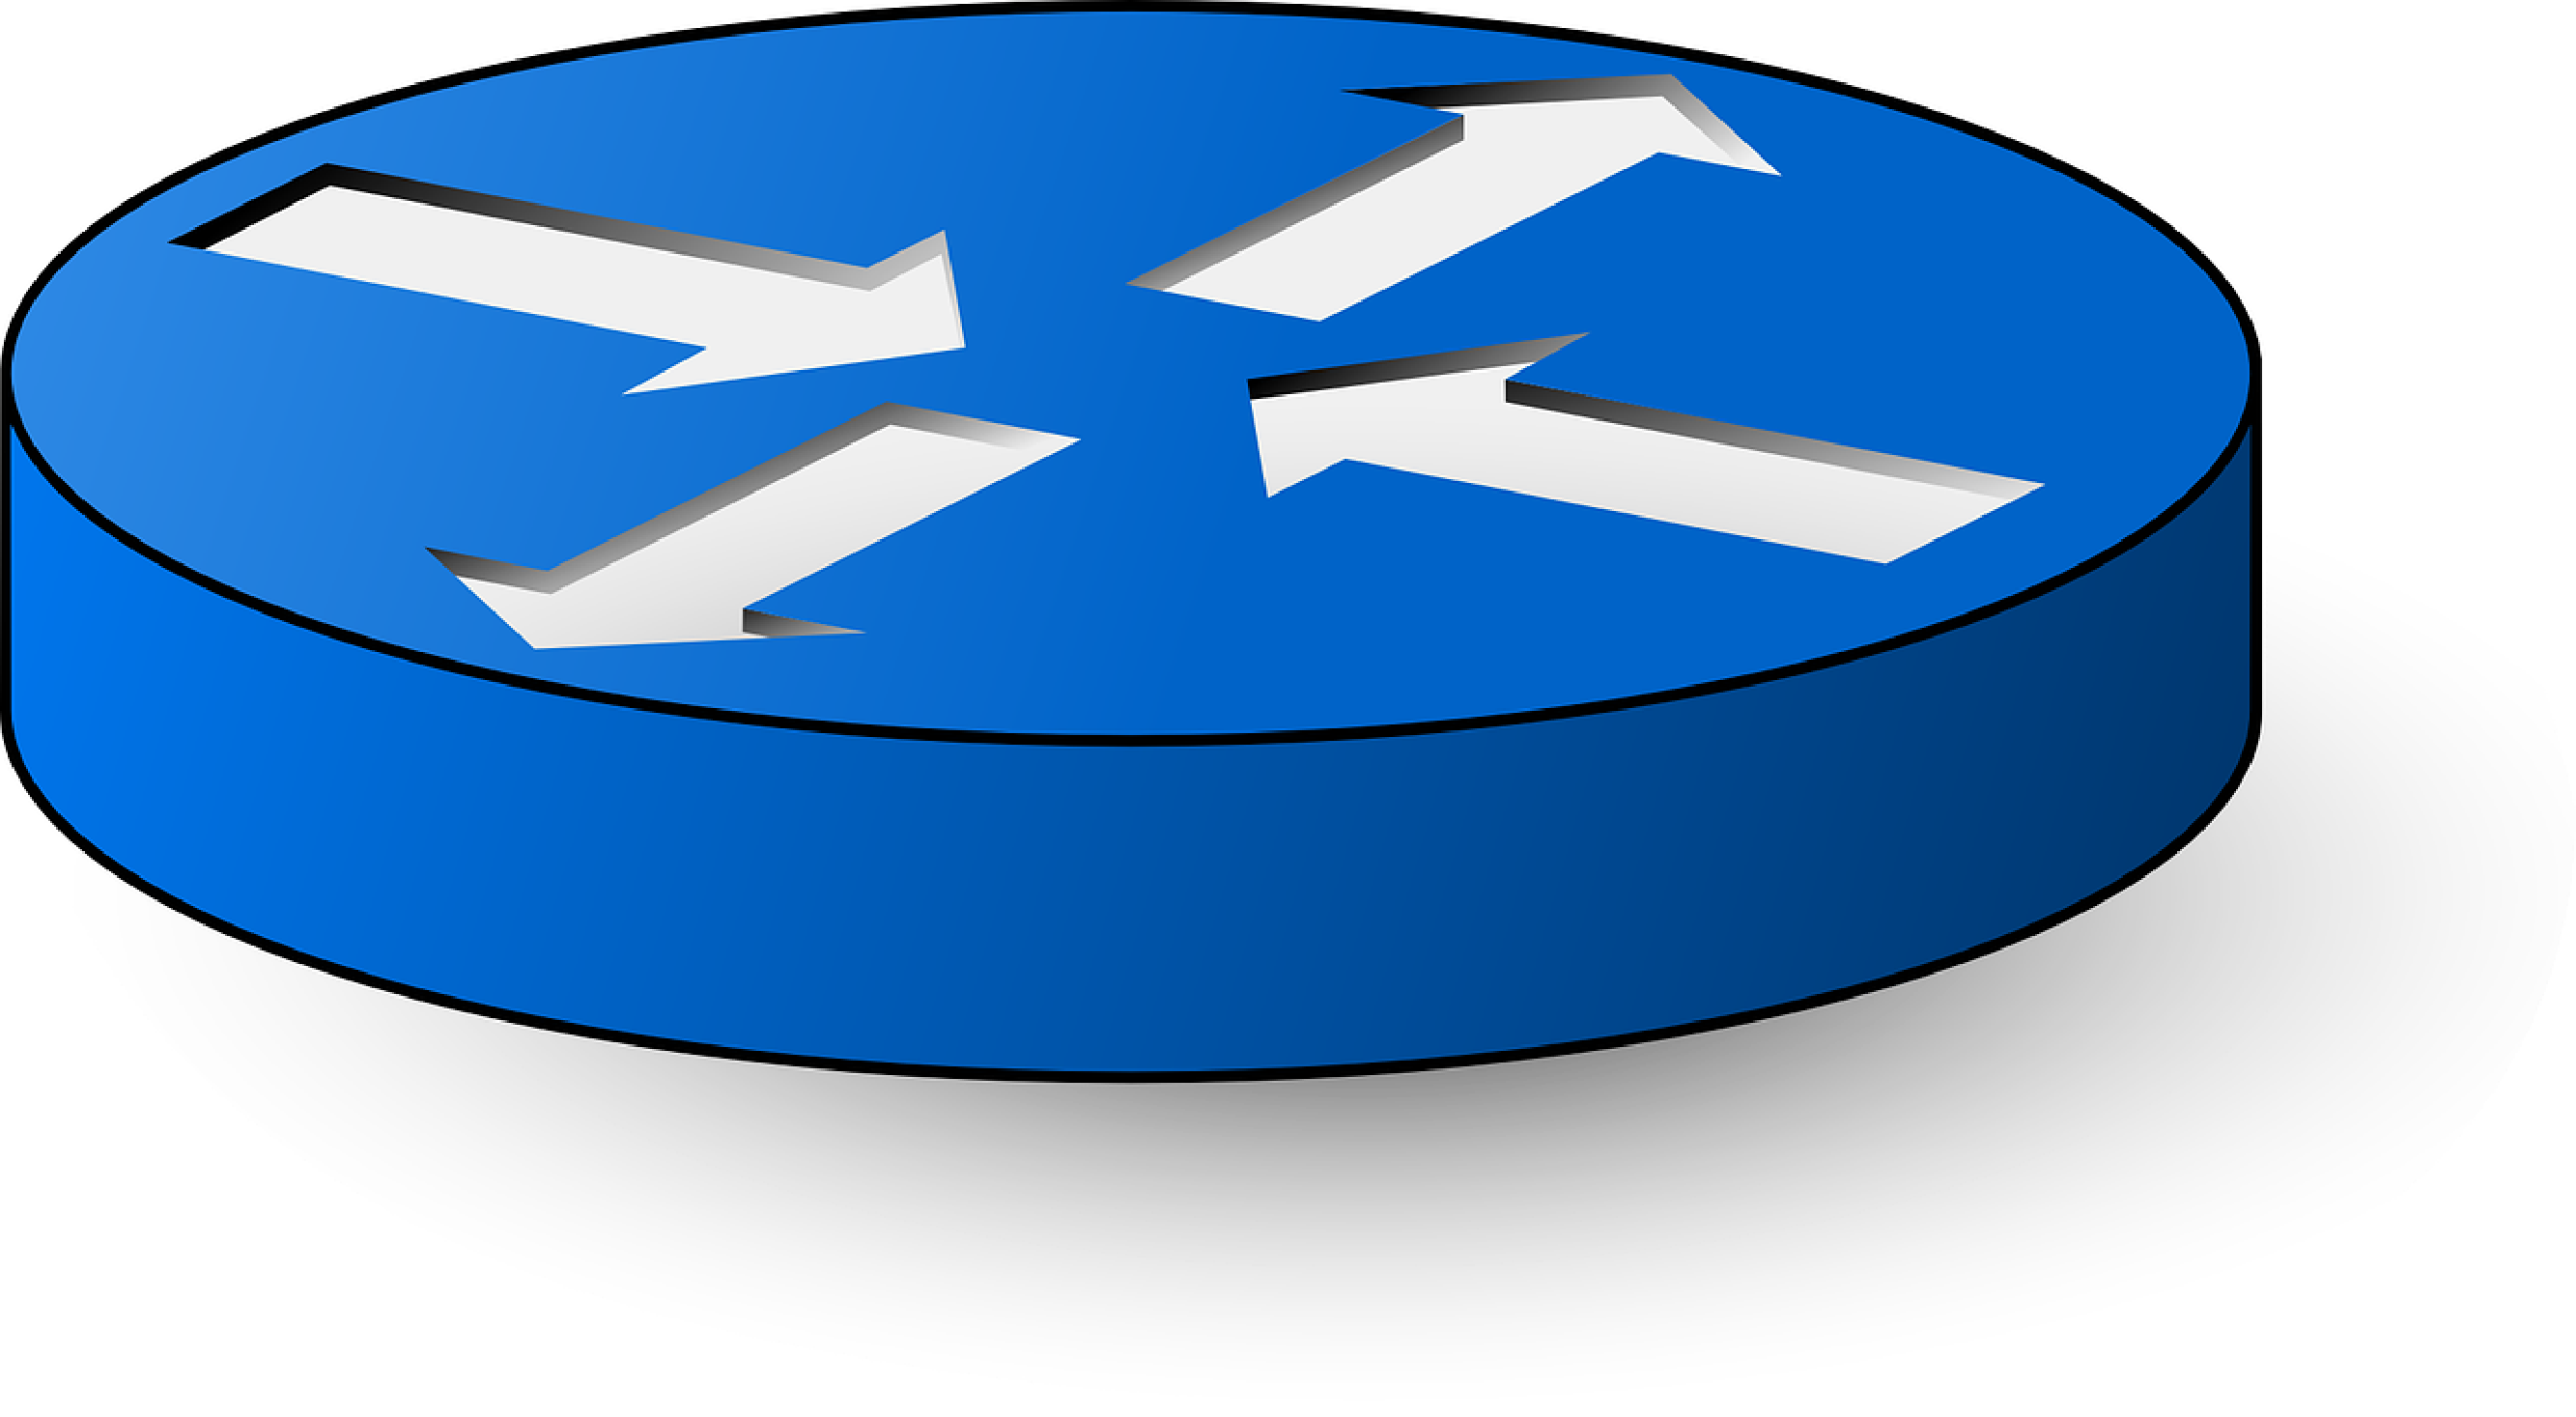
\includegraphics[width=52.5pt,height=52.5pt]{figures/router-30140_1280.pdf}};
%Image [id:dp8562417166935583] 
\draw (200,411.5) node  {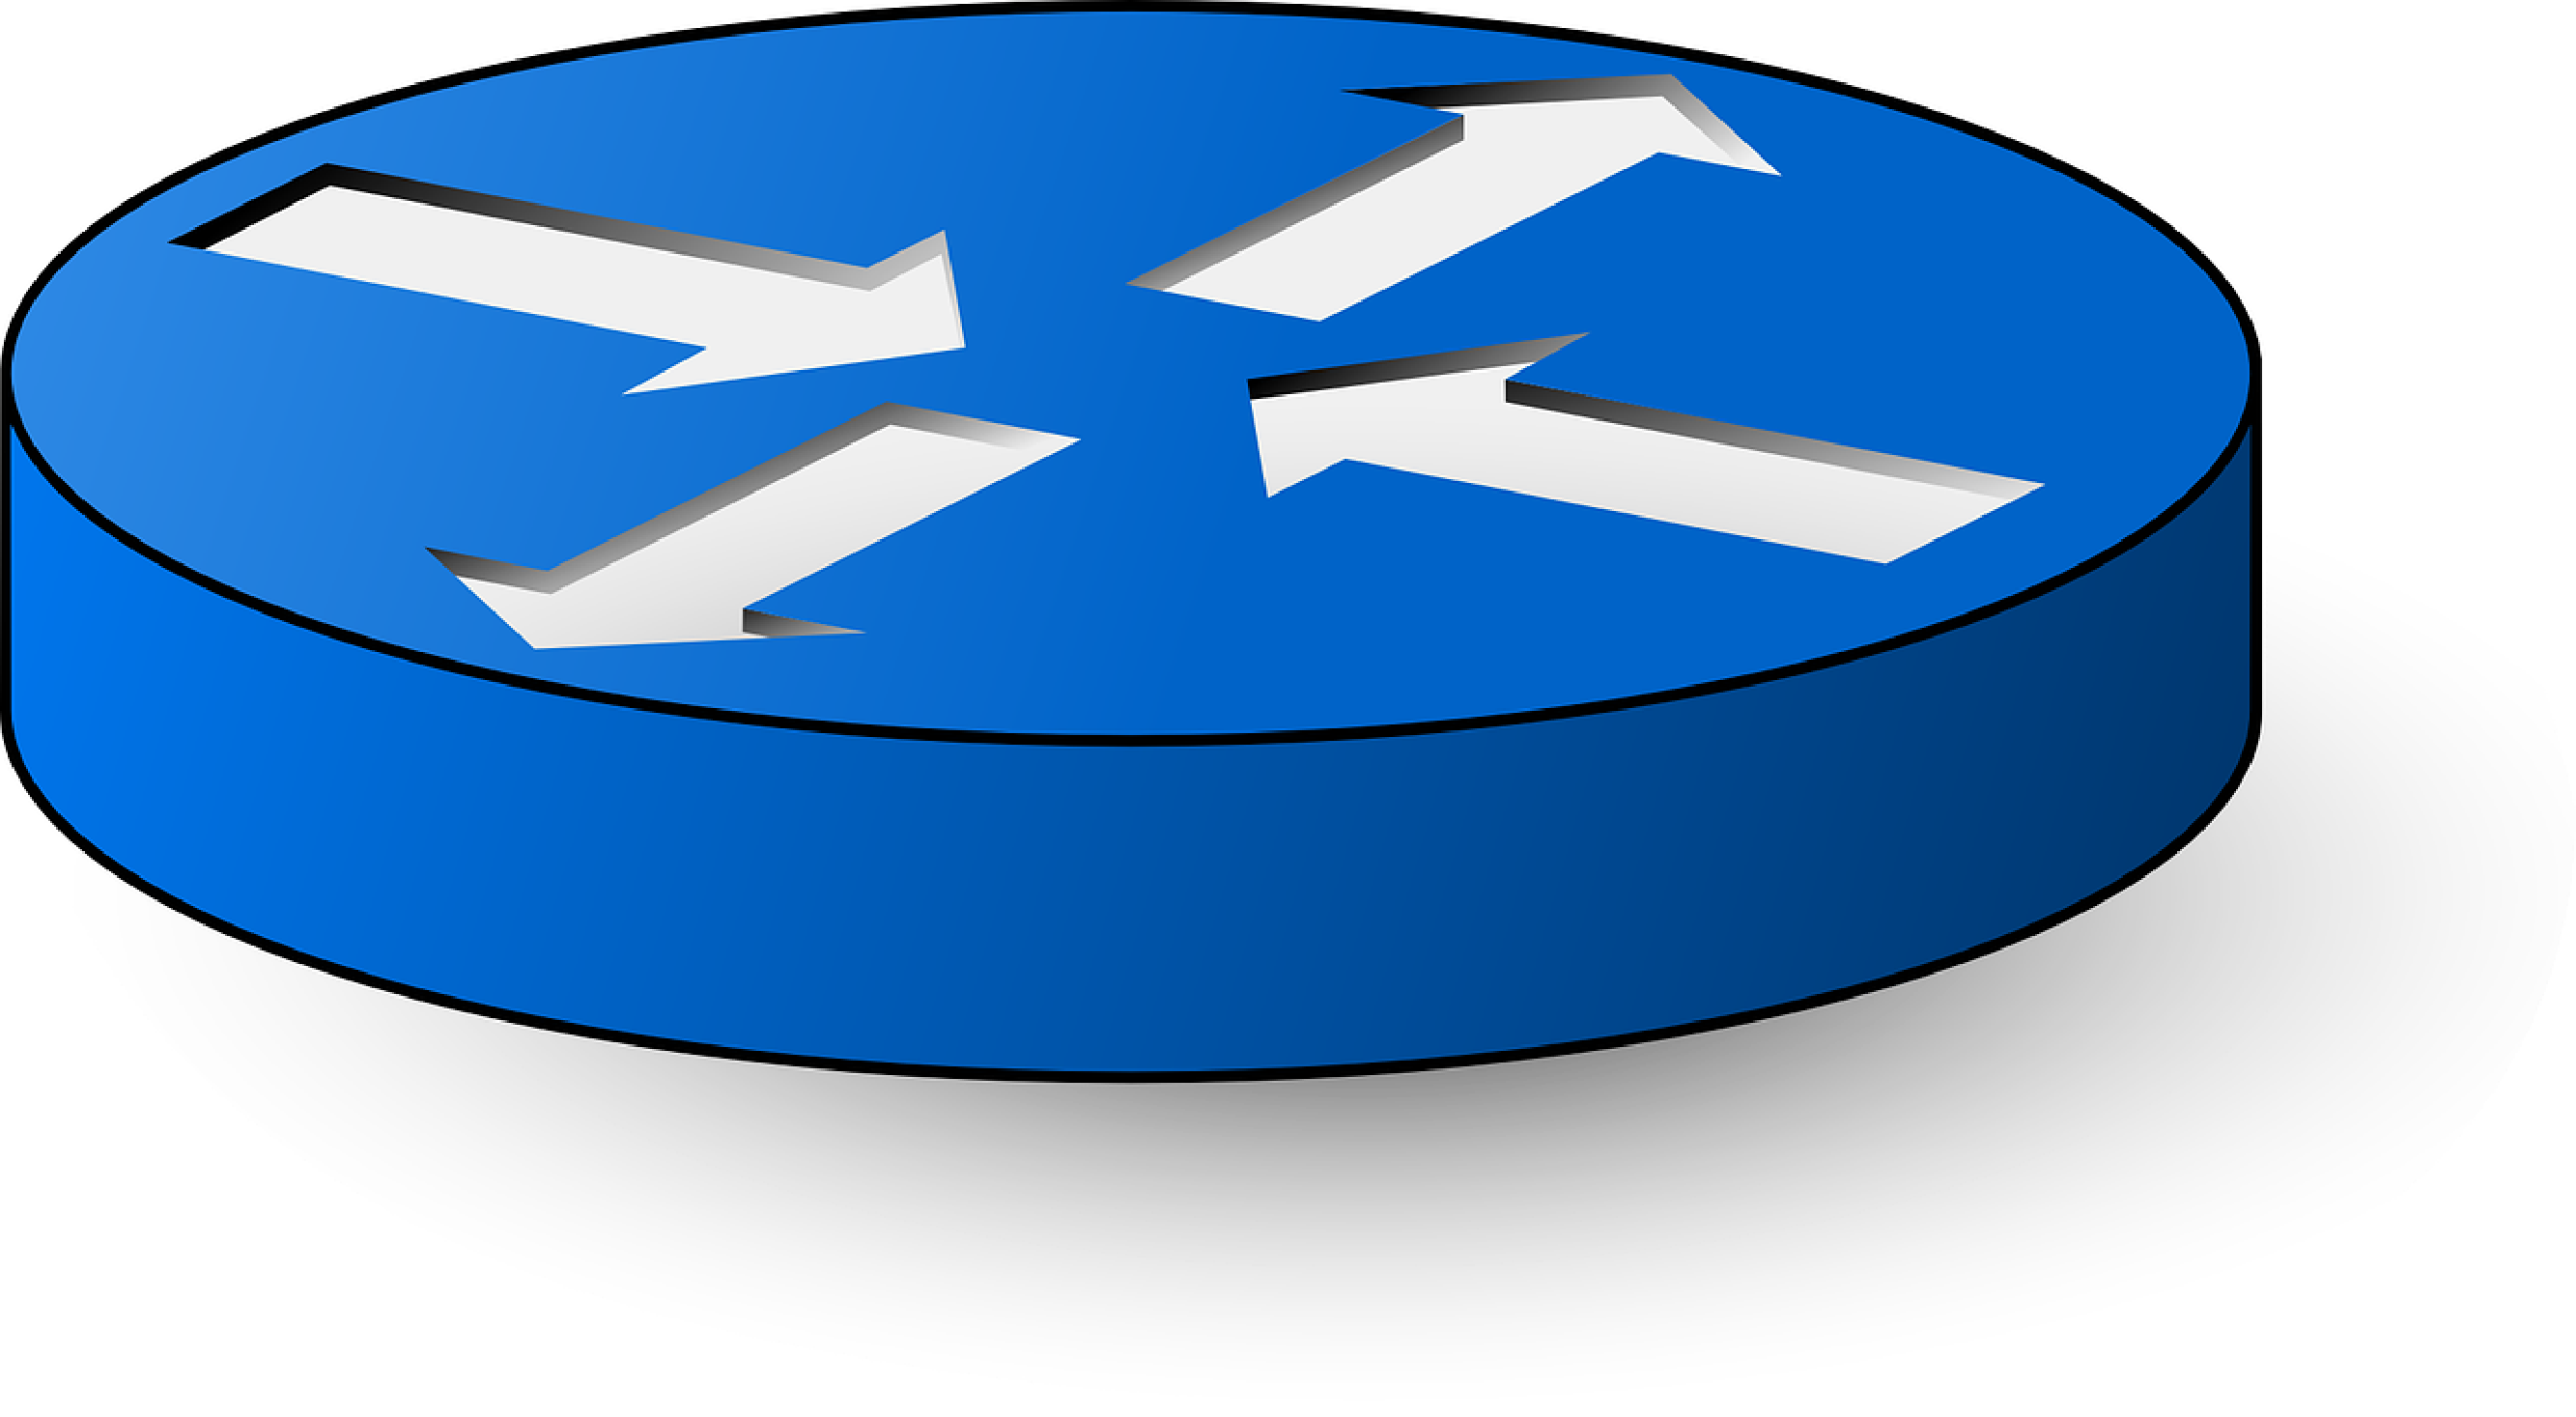
\includegraphics[width=52.5pt,height=52.5pt]{figures/router-30140_1280.pdf}};
%Image [id:dp5197814612037341] 
\draw (312,447.5) node  {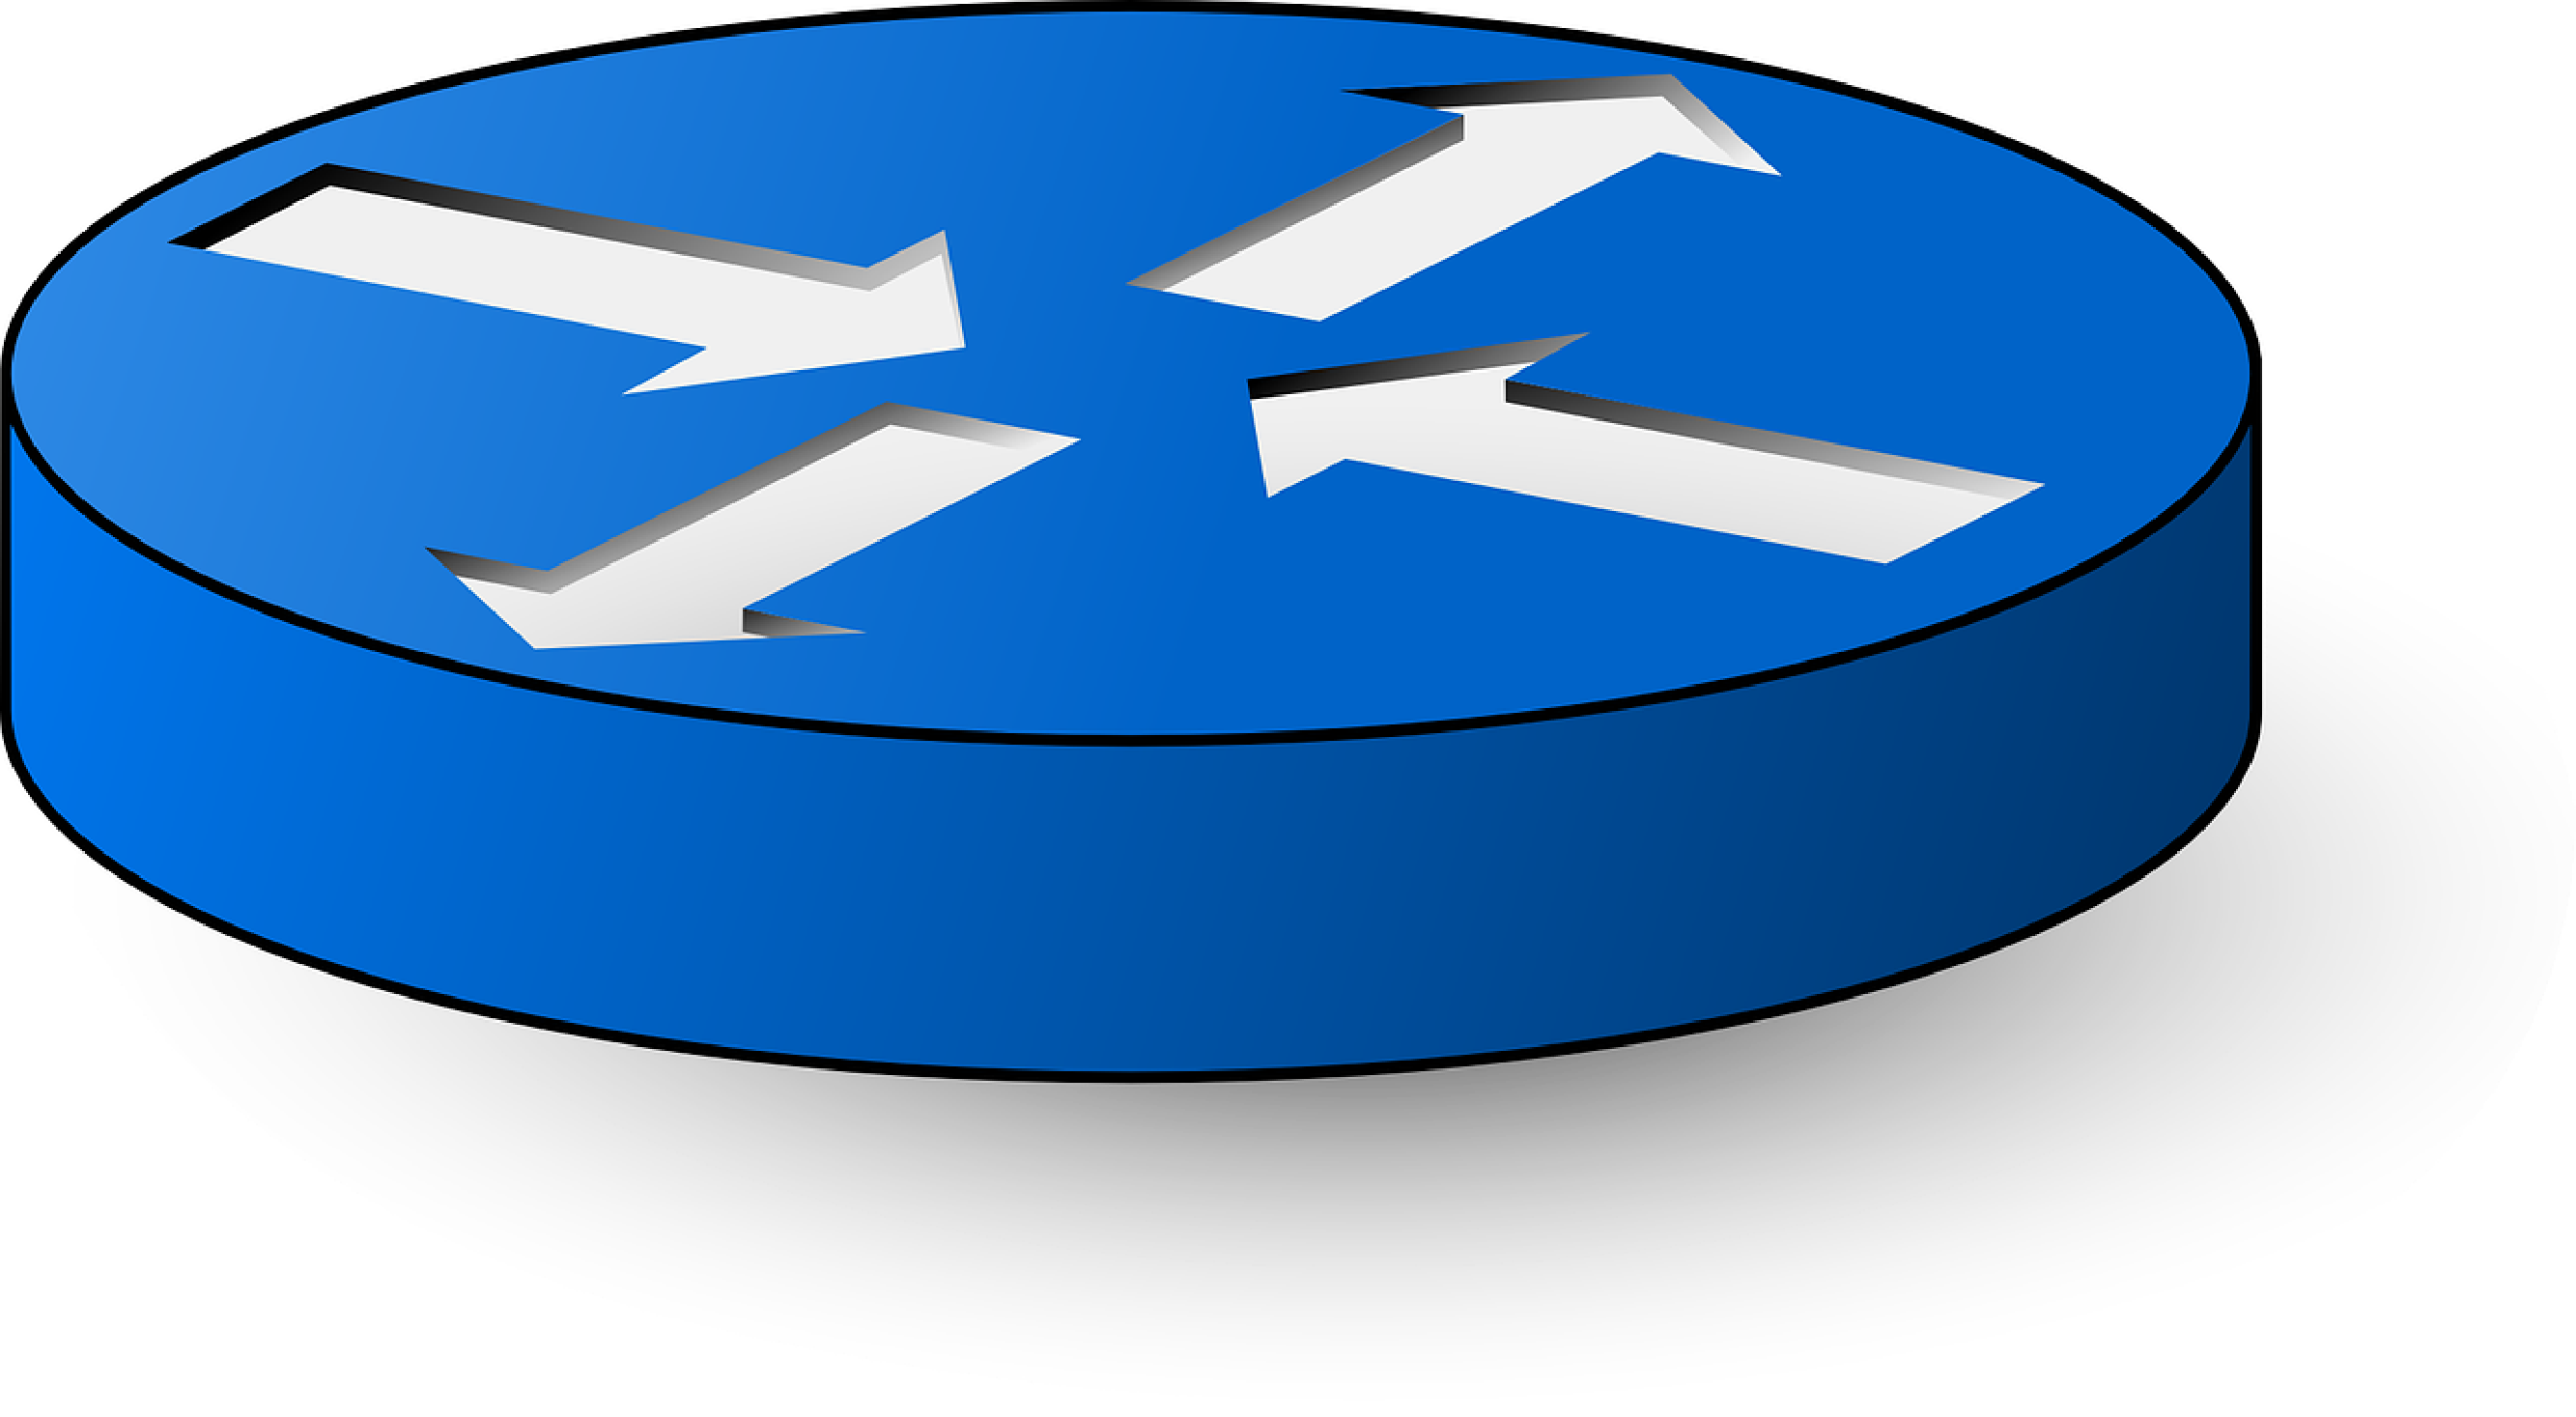
\includegraphics[width=52.5pt,height=52.5pt]{figures/router-30140_1280.pdf}};
%Image [id:dp7997025451564928] 
\draw (461,423.67) node  {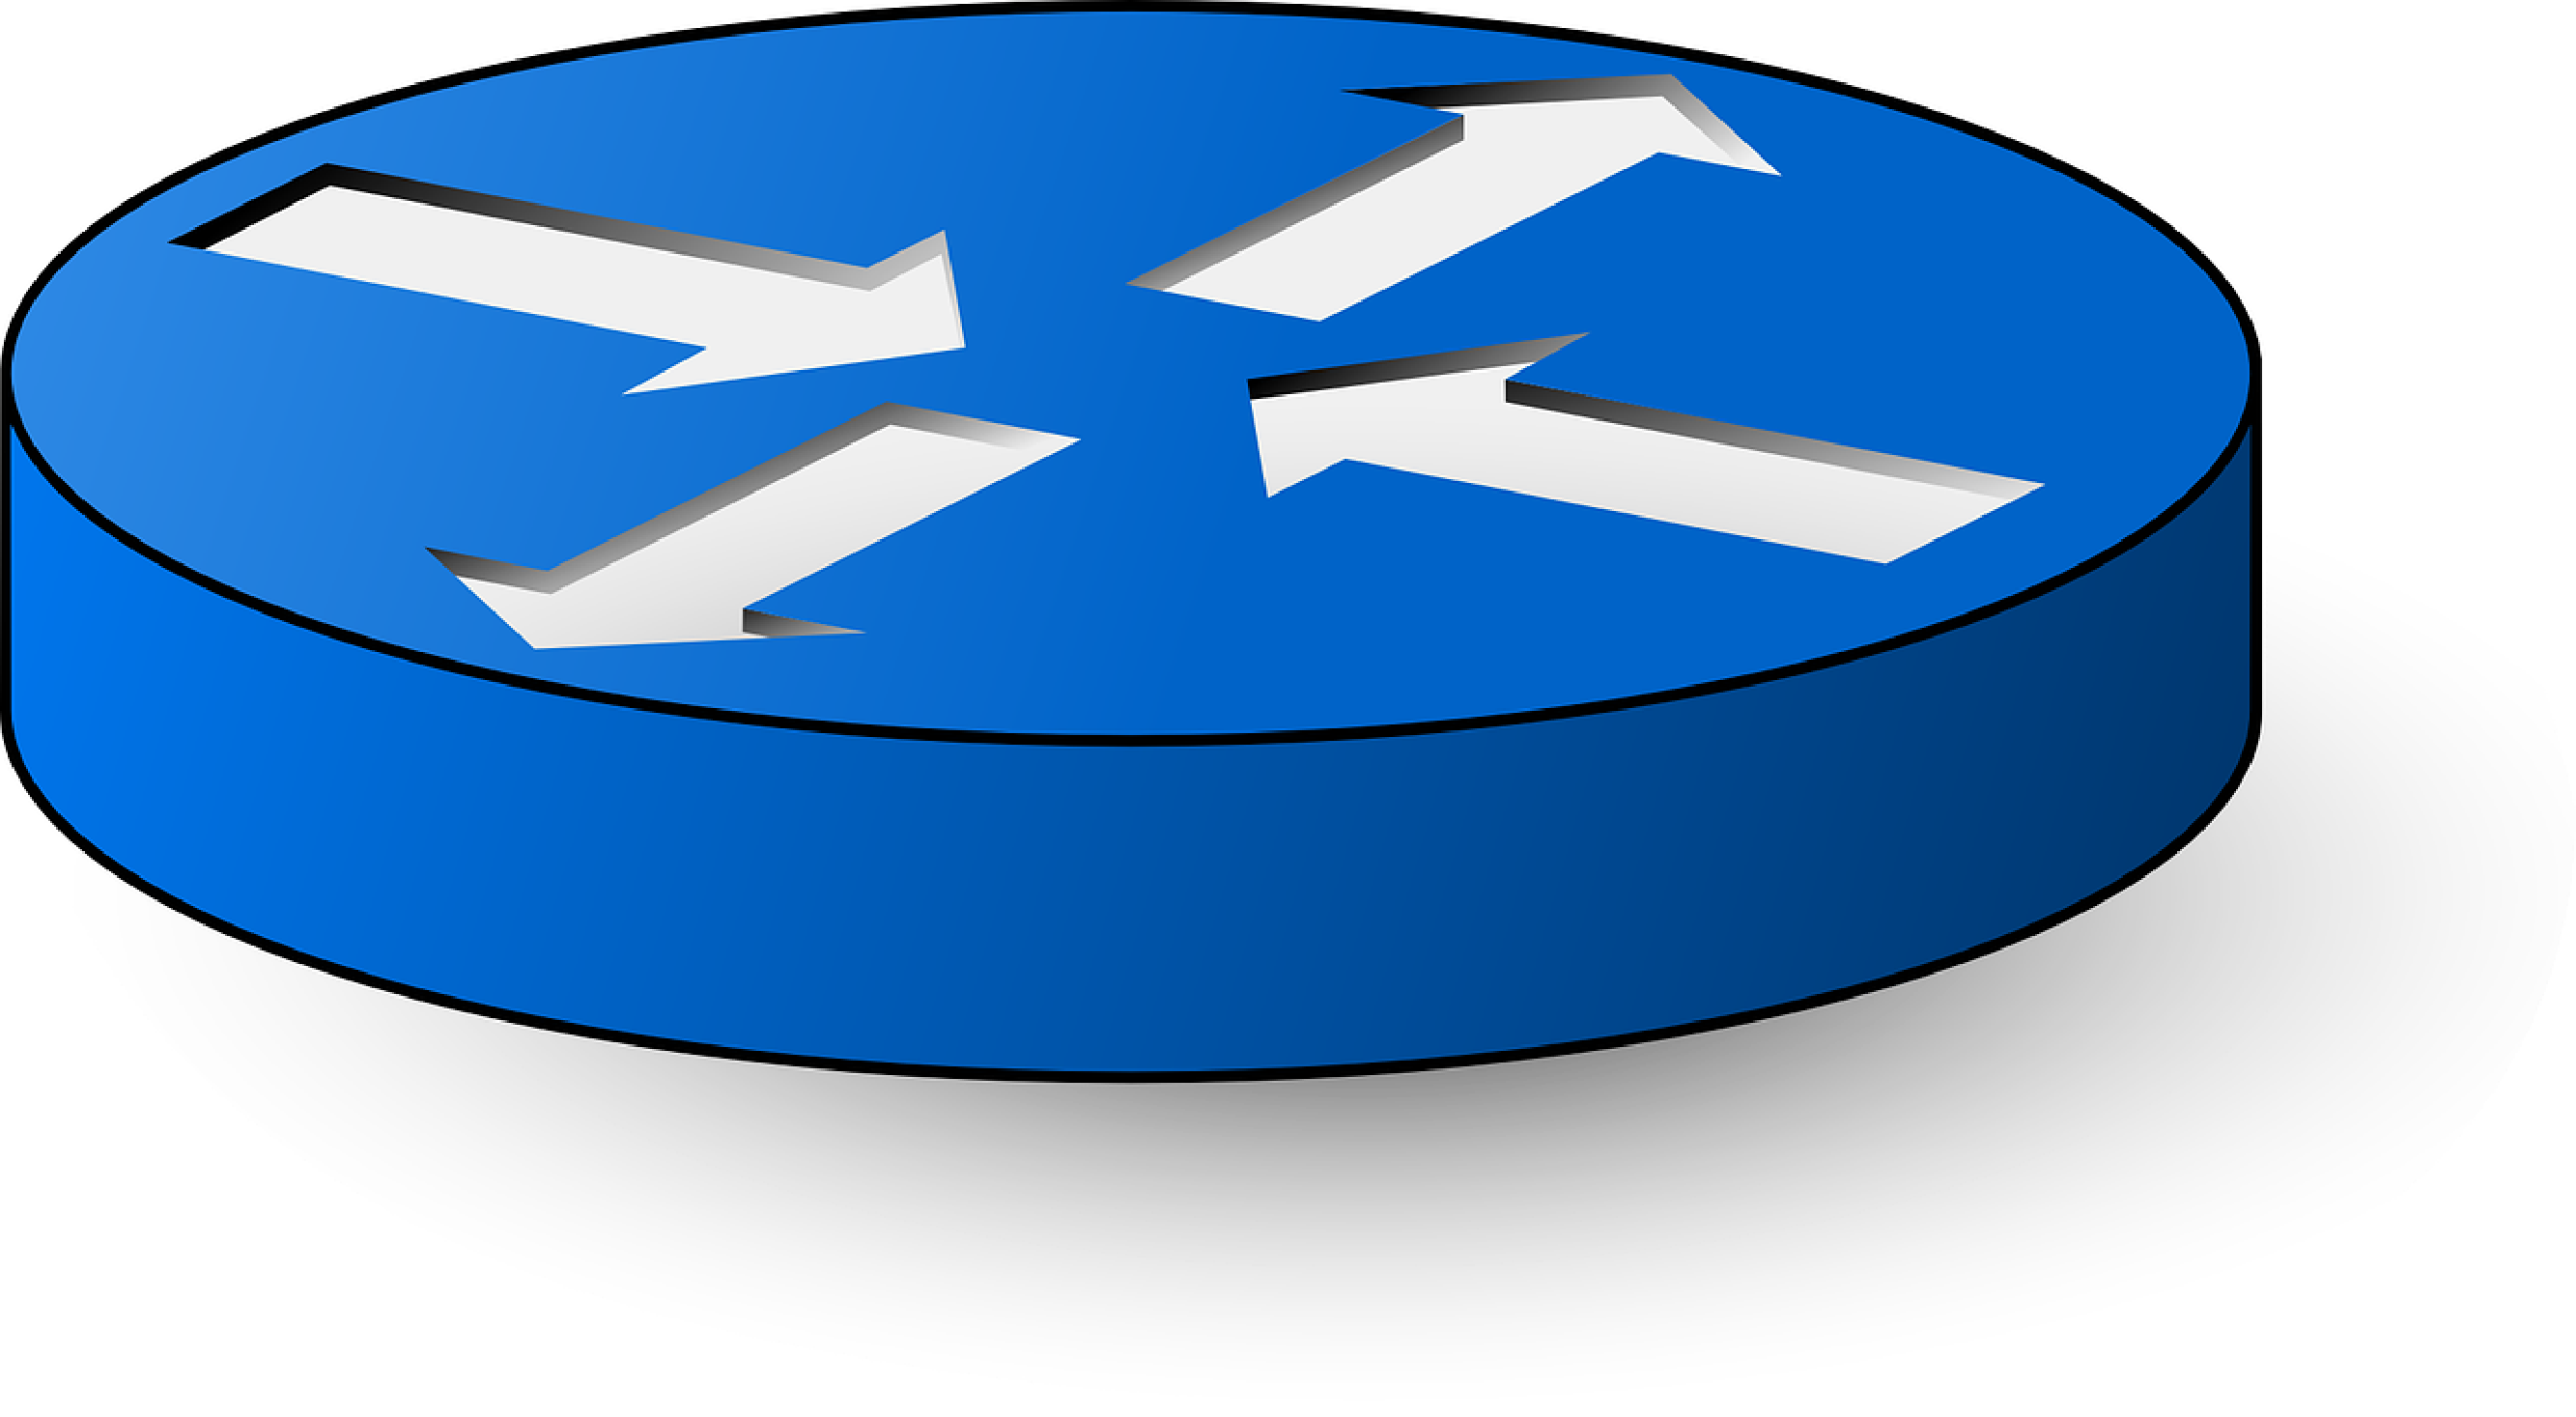
\includegraphics[width=52.5pt,height=52.5pt]{figures/router-30140_1280.pdf}};
%Image [id:dp22576183582057285] 
\draw (453,480.5) node  {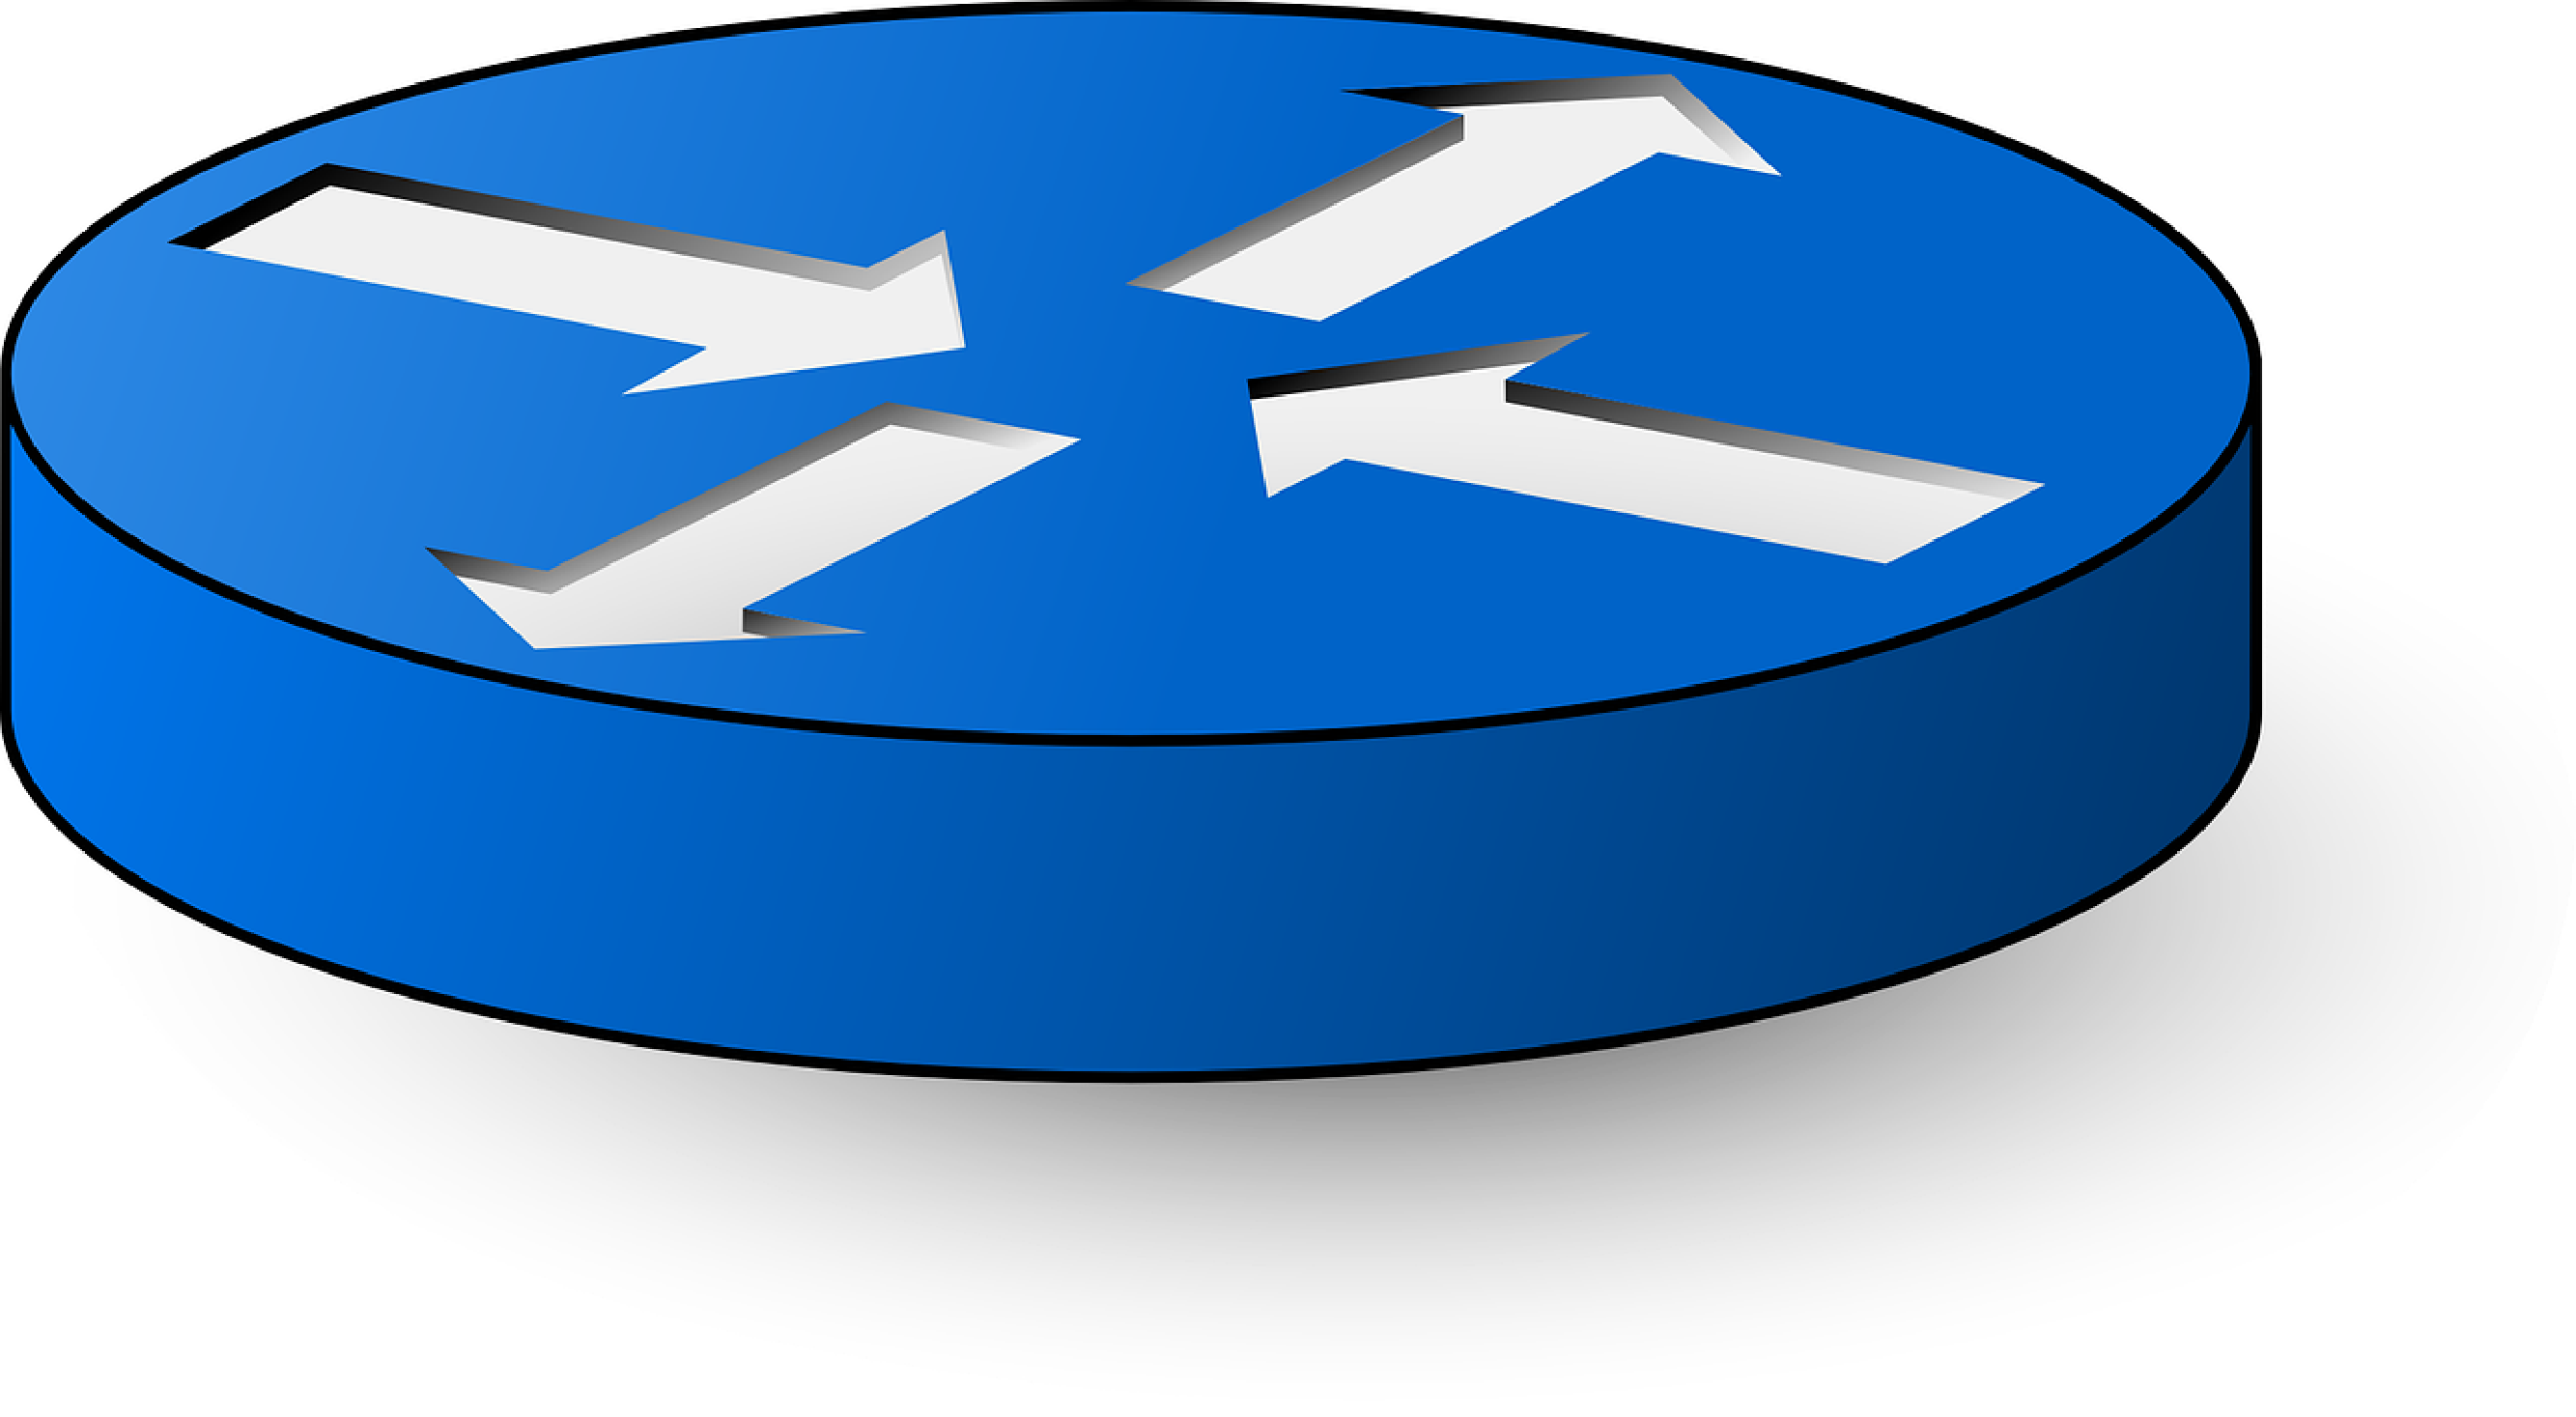
\includegraphics[width=52.5pt,height=52.5pt]{figures/router-30140_1280.pdf}};
%Rounded Rect [id:dp31108656927737066] 
\draw  [fill={rgb, 255:red, 217; green, 154; blue, 232 }  ,fill opacity=1 ] (26,321.78) .. controls (26,316.88) and (29.98,312.9) .. (34.89,312.9) -- (501.11,312.9) .. controls (506.02,312.9) and (510,316.88) .. (510,321.78) -- (510,348.45) .. controls (510,353.35) and (506.02,357.33) .. (501.11,357.33) -- (34.89,357.33) .. controls (29.98,357.33) and (26,353.35) .. (26,348.45) -- cycle ;


% Text Node
\draw (284,495.5) node [scale=0.9] [align=left] {Physical Infrastructure};
% Text Node
\draw (268,335.11) node  [align=left] {Network Hypervisor};
% Text Node
\draw (97,156.5) node [scale=0.9] [align=left] {{\small Virtual Network 1}};
% Text Node
\draw (320,207.5) node [scale=0.9] [align=left] {{\small Virtual Network 2}};


\end{tikzpicture}


\caption{SDN Virtualization}
\label{fig:SDN-hypervisor}
\end{figure}